\documentclass{sig-alternate-05-2015}

\usepackage{url}
\usepackage[table,xcdraw]{xcolor}
\usepackage{listings}
\usepackage{eurosym}
\usepackage{amsfonts}
\usepackage{balance}
\usepackage{cite} %this package is awesome - it reorders lists of citations to be in numeric order
\usepackage{pifont}
\newcommand{\xmark}{\ding{53}}%
\usepackage{eqparbox}
\usepackage{hyperref}
\usepackage{subfigure}
%\usepackage{fancyvrb}

\usepackage{algorithm}% http://ctan.org/pkg/algorithms
\usepackage{algpseudocode}% http://ctan.org/pkg/algorithmicx
\newcommand{\var}[1]{{\ttfamily#1}}% variable

% Tables
\usepackage{booktabs}
\usepackage{pbox}
\renewcommand{\arraystretch}{1.2}
\usepackage{arydshln}
%\renewcommand*\cmidrule{} % No middle lines
%\renewcommand{\arraystretch}{1.5} % Additional spacing with no middle lines
%\renewcommand*\cmidrule{\hdashline[1pt/2pt]}% Dashed middle lines
\renewcommand*\cmidrule{\midrule[0.001em]} % Thin middle lines
%\renewcommand*\cmidrule{\midrule} % Thick middle lines
\newcommand{\todoNow}[1]{\textbf{\textcolor{red}{TODO.NOW: #1}}} %comment out for submission
\newcommand{\todoMid}[1]{\textbf{\textcolor{magenta}{TODO.MID: #1}}} %comment out for submission
%\newcommand{\todoMid}[1]{\textbf{\textcolor{magenta}{}}} %comment out for submission
\newcommand{\todoLast}[1]{\textbf{\textcolor{blue}{TODO.LAST: #1}}} %comment out for submission
\newcommand{\clarify}[1]{{\color{blue}\{CLARIFY: #1\}}}

\usepackage{tikz}
\def\checkmark{\tikz\fill[scale=0.4](0,.35) -- (.25,0) -- (1,.7) -- (.25,.15) -- cycle;}



%Images
%\usepackage[pdftex]{graphicx}
\DeclareGraphicsExtensions{.pdf,.jpg,.png}

\hyphenation{second-ly ap-pen-dix}

\clubpenalty = 10000
\widowpenalty = 10000
\displaywidowpenalty = 10000

\newcommand{\horiz}{\hspace{2.1pt}}
\renewcommand{\topfraction}{.9}

\newcommand{\ignore}[1]{}

\begin{document}
%\bstctlcite{IEEEexample:BSTcontrol}
%
% paper title
% can use linebreaks \\ within to get better formatting as desired
\title{Refactoring Regular Expressions}


\numberofauthors{2}
\author{
% 1st. author
\alignauthor
Carl Chapman\\
       \affaddr{Department of Computer Science}\\
       \affaddr{Iowa State University}\\
       \email{carl1976@iastate.edu}
\alignauthor
Kathryn T. Stolee\\
       \affaddr{Department of Computer Science}\\
       \affaddr{North Carolina State University}\\
       \email{ktstolee@ncsu.edu}
\alignauthor
}


\maketitle


\begin{abstract}
Regular expressions (regex) are powerful tools employed across many tasks and platforms.
Regex can be complex, so optimizing understandability of regex is desirable for maintainers.
Because of a rich feature set, there is more than one way to compose a regex to get the same desired behavior.
We define five equivalence classes where the same behavior can be achieved with multiple representations.
With the goal of finding refactorings that improve understandability, we analyze regexes in GitHub to find community standards, and obtain understandability metrics from an empirical study with 180 participants to find out which representations are more  understandable to programmers.
We found, for example, that patterns requiring one or more of some character expressed using kleene star such as \verb!`::*'! are more understandable when expressed using the plus: \verb!`:+'!.  We identify strongly preferred transformations in three of the five equivalence classes and identify opportunities for future work in improving regex refactoring. 
%
%as well as other, less conclusive information that can inform future investigation into regex refactoring.

\end{abstract}

\section{Introduction }

Regular expressions (regexes) are used fundamentally in string searching and substitution tasks, such as word searching, text editing, file parsing, user input validation, and access controls. More advanced uses can be seen in search engines~\cite{zhao2005fully}, database querying~\cite{Yeole:2011:ADT:1980022.1980229}, and network security~\cite{network,hutchings2002assisting,ficara2008improved}.

Recent research has suggested that regular expressions are hard to understand, hard to compose, and error prone~\cite{Spishak:2012:TSR:2318202.2318207}. Given their frequent appearances in software source code and the difficulty of working with them, some effort has been put into easing the burden on developers by providing environments that make regexes easier to understand. Some tools provide debugging environments which explain string matching results and highlight the parts of regex patterns which match a certain string~\cite{regex101, regexr}. Other tools present graphical representations (e.g., finite automata) of the regular expressions~\cite{regexper, rise4fun}. Still, others can automatically generate strings according to a given regular expression~\cite{hampi, rex} or automatically generate regexes according to a given list of strings~\cite{Babbar:2010:CBA:1871840.1871848, Li:2008:REL:1613715.1613719}.
%why we need analysis despite the tools
%While these tools are helpful, there are some restrictions which hinder their usage. They may need the regex and a matched string at the same time, do not support some commonly used regular expression features, generate non-printable strings, or generate an overfitted regular expressions.
The commonality of such tools and techniques provides evidence that developers need help with regex composition and comprehension.

In software engineering, code smells have been found to hinder understandability of source code~\cite{abbes2011empirical, du2006does}.
Once removed through refactoring, the code becomes more understandable, easing the burden on the programmer.
In regular expressions, such code smells have not yet been defined, perhaps in part because it is not clear what makes a regex difficult to understand or maintain.
This is one of the goals of this work, to explore language features that impact comprehension and begin to identify code smells in regexes.

In regular expressions as in source code, there are multiple ways to express the same semantic concept.
For example, the regex, \verb!aa*! matches an ``a" followed by zero or more ``a", and is equivalent to \verb!a+! , which matches one or more ``a".
That is, both regexes match the same \emph{language} but are expressed using different syntax. What is not clear is which representation, \verb!aa*! or \verb!a+!, is more easily understood.
%Preferences in regex refactorings could vary, including which is easier to maintain, easier to understand, or better conforms to community standards, depending on the goals of the programmer.

In this work, we focus on identifying regex comprehension smells.
We identify equivalence classes of regex representations that provide options for concepts such as double-bounds in repetitions (e.g., \verb!a{1,2}!, \verb!a|aa!) or
%single-bounds in repetitions (e.g., \verb!`a{2}'! or \verb!`aa'!),
%lower bounds in repetitions (e.g., \verb!`a{2,}'! or \verb!`aaa*'!),
character classes (e.g., \verb![0-9]!, \verb![\d]!).
%, and literals (e.g., \verb!`\a'! or \verb!`\x07'!).
Based on an empirical study measuring regex comprehension on 42 pairs of regexes using 180 participants, as well as an empirical study of nearly 14,000 regexes and their features, we identify smelly and non-smelly regex representations. For example, \verb!aa*! is more smelly than \verb!a+!, based on feature usage frequency in source code (conformance to community standards) and understandability.
%Our results identify preferred representations for four of the five types of equivalence classes based on mutual agreement between community standards and understandability. For the fifth group on double-bounded repetitions, two recommendations are given depending on the programmer's goals.
Our contributions are:

\vspace{-3pt}
\begin{itemize}
\item An empirical study to evaluate regex comprehension with 180 participants for studying regex understandability,
\item Identification of five equivalence classes and 18 corresponding representations for regular expressions, and
%\item Conducted an empirical study identifying opportunities for regex refactoring in Python projects based on how regexes are expressed,
\item Identification of smelly and non-smelly regex representations to optimize 1) understandability and 2) conformance to community standards, backed by empirical evidence.
%\item {Identified 3 or so other regex refactorings categories and specific instances that are worthy of further investigations}
%\item {Identified a few regex refactorings that can be eliminated because both options are equally readable}
\end{itemize}
\vspace{-3pt}

Despite the frequent usage of regexes in source code~\cite{chapman2016}, this is the first work to explore regex comprehension.
%We approach the problem of identifying preferred regex representations by looking at thousands of regexes in Python projects and measuring comprehension using human participants. %, one using source code artifacts and another using human participants.
%The rest of this paper is structured as follows:
%Section~\ref{sec:study} presents the research questions and high-level study designs.
%Section~\ref{sec:refactoring} describes the equivalence classes explored for regex smell detection.
%Section~\ref{sec:rq1} presents the results for RQ1 about comprehension code smells,
%Section~\ref{sec:rq2} presents the results of RQ2 on community standards code smells, and
%Section~\ref{sec:rq3} looks at the preferred representations.
%Section~\ref{sec:discussion} discusses the implications of our results and the future work, followed by related work in Section~\ref{sec:related} and the conclusion in Section~\ref{sec:conclusion}.
%Section~\ref{sec:discussion} discusses future work, followed by related work in Section~\ref{sec:related} and the conclusion in Section~\ref{sec:conclusion}.
% (Section~\ref{sec:refactoring}), research questions (Section~\ref{sec:study}), the study of regex representations in Python projects (Section~\ref{communitystudy}), and the regex understandability study using human participants (Section~\ref{sec:understandability}). We discuss the overall analysis results in Section~\ref{sec:rq3}, implications in Section~\ref{sec:discussion}, related work in regexes (Section~\ref{sec:related}), and conclude in Section~\ref{sec:conclusion}.
%\todoLast{can remove for space}
%The rest of this paper is organized as follows:
%We define the research questions in Section~\ref{} followed by an explanation of the equivalence classes in Section~\ref{}. The study design and results for RQ1 are in Section~\ref{} followed by the study design and results for RQ2 in Section~\ref{}. RQ3 is in Section~\ref{}, the discussion is in Section~\ref{}, related work is in Section~\ref{}, and the conclusion is in Section~\ref{}.
%
%Related work, study, results, discussion, conclusion.


\begin{figure*}[tb]
\centering
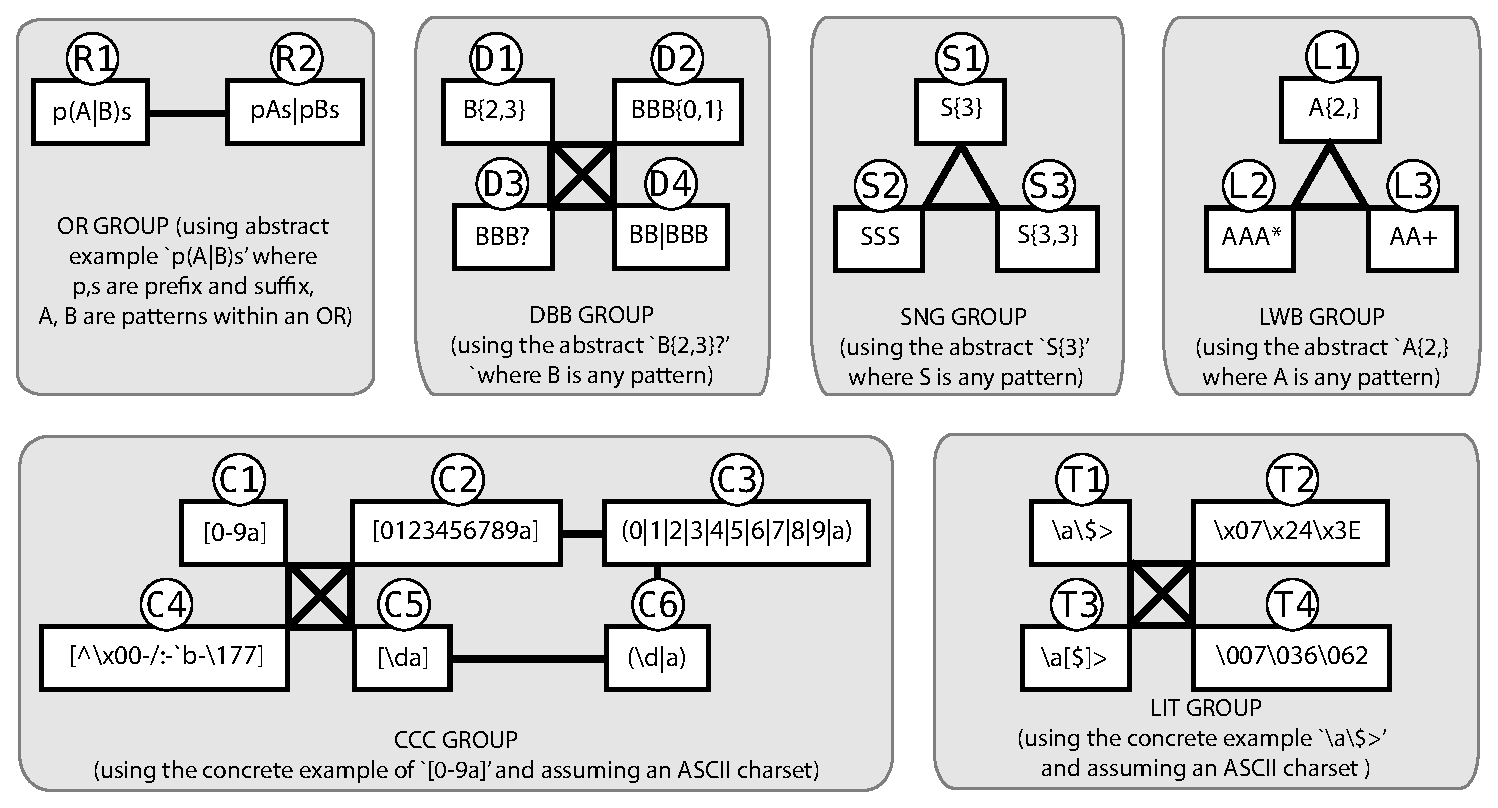
\includegraphics[width=\textwidth]{illustrations/refactoringTree.eps}
%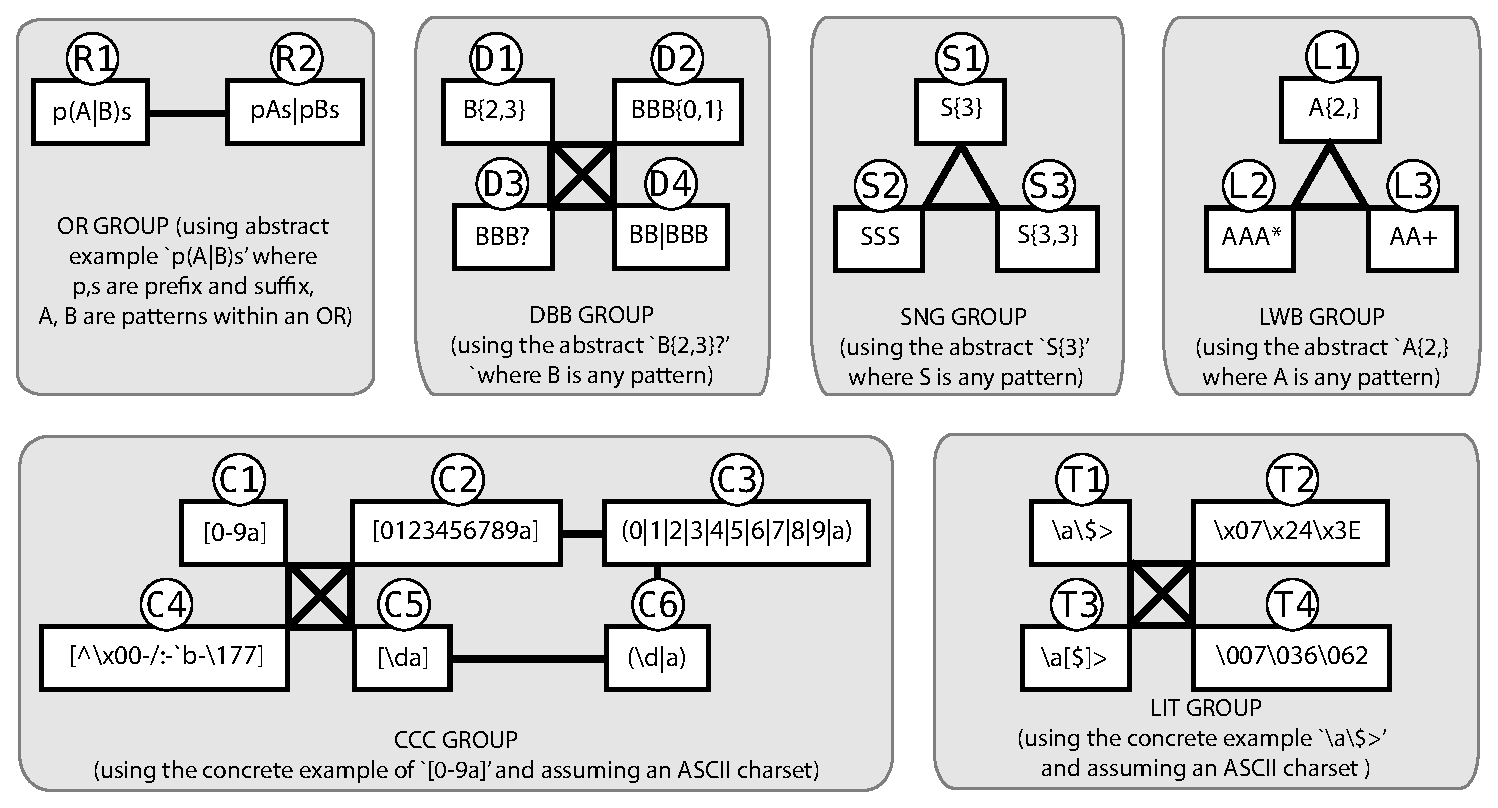
\includegraphics[scale=0.8]{illustrations/refactoringTree.eps}
%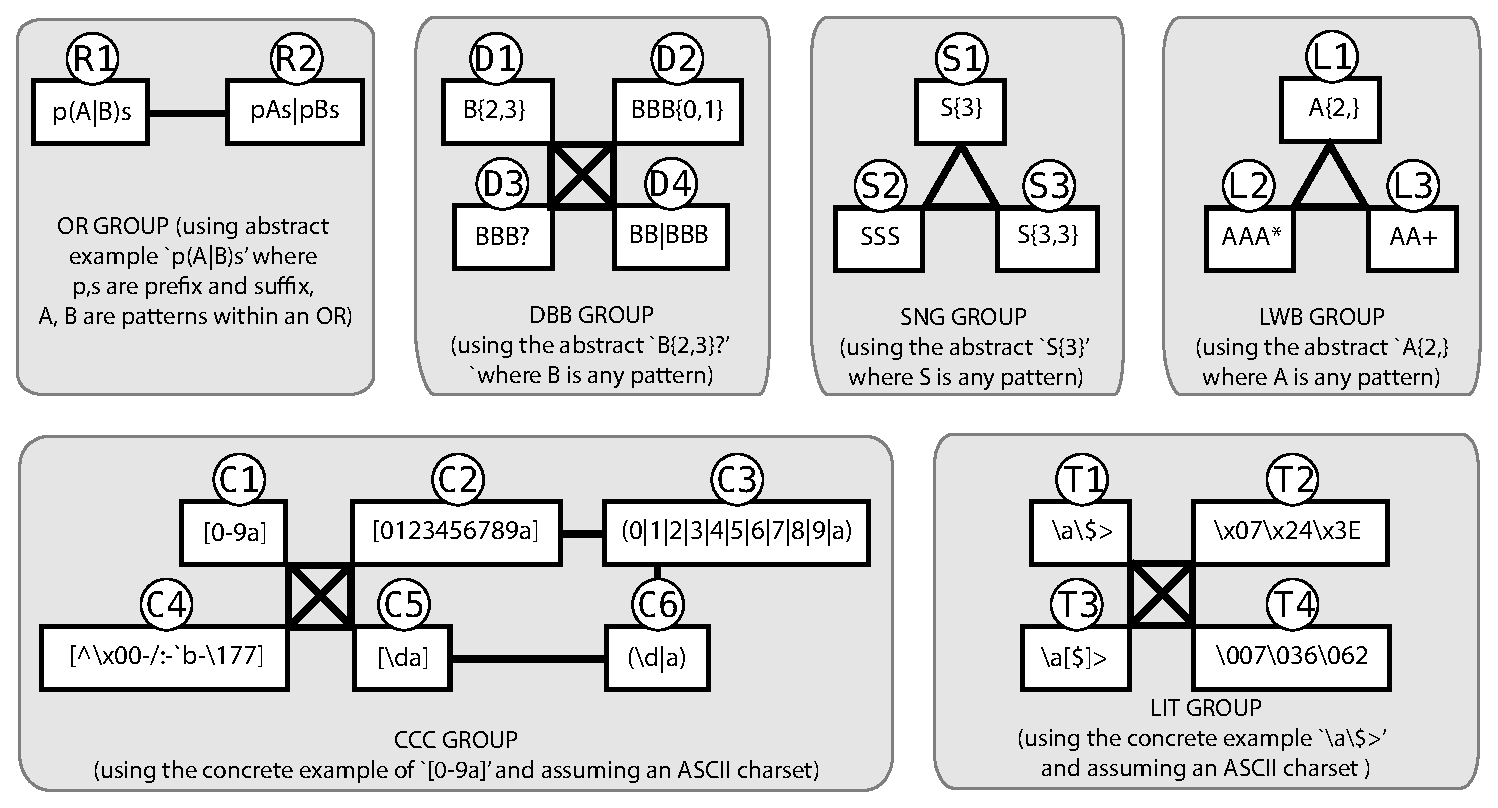
\includegraphics[width=0.85\textwidth]{illustrations/refactoringTree.eps}
\vspace{-6pt}
\caption{Equivalence classes with various representations. DBB = Double-Bounded, SNG = Single Bounded, LWB = Lower Bounded, CCC = Custom Character Class and LIT = Literal. We use concrete regexes along with their Deterministic Finite Automaton (DFA) in the representations for illustration. However, the A's in the LWB group (or B's in DBB group, S's in SNG group, and so forth) abstractly represent any pattern that could be operated on by a repetition modifier (e.g., literal characters, character classes, or groups). The same is true for the literals used in all the representations. }
\vspace{-6pt}
\label{fig:refactoringTree}
\end{figure*}


\section{Research Questions}
\label{sec:study}
%After defining the equivalence classes and potential  regex refactorings as described in Section~\ref{sec:refactoring}, we wanted to know which representations in the equivalence classes  are considered desirable and which might be smelly. Desirability for regexes can be defined many ways, including maintainable,  understandable, and performance.
%%As prior work has shown that regexes are difficult to read~\cite{},
%We focus on refactoring for understandability.

To explore regex comprehension and identify smells, we answer the following research questions: \\
%We define regex understandability two ways. First,  we  present people with regexes exemplifying some of the more common characteristics and ask them comprehension questions along two directions: determine which of a list of strings are matched by the regex, and compose a string that is matched by the regex. Second, assuming that common programming practices are more understandable than uncommon practices, we explore the frequencies of each representation from Figure~\ref{fig:refactoringTree} using thousands of regexes scraped from Python projects.

\noindent {\textbf{RQ1:}} {\em Which regex representations are most understandable?}
To answer RQ1, we conduct a study in which programmers are presented with a regex and asked comprehension questions about its matching behavior.  By comparing accuracy between regexes that match the same language but are expressed differently (e.g., \verb!tri[a-f]3! and \verb!tri(a|b|c|d|e|f)3!), we can measure understandability and identify code smells. We also explore at the relationship between regex comprehension and regex size, as measured by string length and the DFA built for each regex.

This analysis requires identification of equivalence classes for regexes. By inspecting  nearly 14,000 regexes extracted from Python projects in a publicly available dataset~\cite{chapman2016}, we formed an initial set of five equivalence classes to explore. \\
% as measured by identifying matching strings and by composing matching strings

\noindent {\textbf{RQ2:}} {\em Which regex representations have the strongest {community support} based on  frequency?} % each representation appears in regexes in open source Python projects?}
To answer RQ2, we explore the publicly available regex dataset~\cite{chapman2016} and use the presence and absence of language features as a proxy for community support, where more frequently-used features are assumed to be more understandable.\\

\noindent {\textbf{RQ3:}}  {\em Which regex representations are most desirable (i.e., least smelly) based on both community support and understandability?}
Based on RQ1 and RQ2, we identify smelly and non-smelly regex features  based on a combination of comprehension metrics and community support. \\

Next, we present the equivalence classes, analysis and results for each RQ, and a unified discussion.







%\footnote{same dataset used in prior work~\cite{chapman2016}}
\section{Equivalence Classes}
\label{sec:refactoring}
%After studying over 13,000 distinct regex strings from Python projects, 
To explore understandability, we defined an initial set of equivalence classes for regexes. 
Using the publicly available behavioral clusters of Python regexes~\cite{chapman2016}, we manually identified several representations that appeared in many of the larger clusters. 
While not a complete set of equivalence classes, this is the first work to explore regex  understandability, and these equivalence classes provide an initial testbed for exploration.
% (Section~\ref{sec:futureequivclasses} identifies other equivalence classes left to explore in future work.)

%For example,  \verb!AAA*! and \verb!AA+! are semantically identical, except one uses the star operator (indicating zero or more repetitions) and the other uses the plus operator (indicating one or more repetitions).
%Both match strings with two or more \verb!A!'s.
Figure~\ref{fig:refactoringTree} shows five equivalence classes in grey boxes and semantically equivalent \emph{representations} in white boxes with identifiers in white circles. For example, LWB is an equivalence class with representations L1, L2, and L3. Regexes \verb!AAA*! and \verb!AA+!  map to L2 and L3, respectively.
%, along with the L1 representation, \verb!A{2,}!.
%The undirected edges between the representations define possible refactorings.
%Identifying the best direction for each arrow in the possible refactorings is discussed in Section~\ref{sec:rq3}.
%We use concrete regexes in the representations to more clearly illustrate examples of the representations. However, the \verb!A!'s in the LWB group abstractly represent any pattern that could be operated on by a repetition modifier (e.g., literal characters, character classes, or groups). The same is true for the literals used in all the representations. 
Next, we describe each equivalence class group. 

\subsection{Custom Character Class Group}
The Custom Character Class (CCC) group has regex representations that use the custom character class language feature or can be represented by such a feature.
%The character class regex language feature is a fundamental feature found in all language flavors since GREP (check this?).
 A custom character class matches a set of alternative characters.  For example, the regex \verb!c[ao]t! will match strings ``cat" and ``cot" because, between the \verb!c! and \verb!t!, there is a custom character class, \verb![ao]!, that specifies either \verb!a! or \verb!o! (but not both) must be selected.  We use the term \emph{custom} to differentiate these classes  from the default character classes, : \verb!\d!, \verb!\D!, \verb!\w!, \verb!\W!, \verb!\s!, \verb!\S! and \verb!.!,  provided by most regex libraries, though the default classes can be encapsulated in a custom character class. %, as is the case with the C4 representation.
 % For the purposes of our analysis, a negated custom character class (like \verb![^abc]!) is handled separately.
%Next, we provide descriptions of each representation in this equivalence class:
\begin{description}  \itemsep -1pt
\item[C1:] Any pattern that contains a (non-negative) custom character class with  a range feature like \verb![a-f]! as shorthand for all of the characters between `a' and `f' (inclusive) belongs to  C1.


\item[C2:] Any pattern that contains a (non-negative) custom character class  without any shorthand representations, specifically ranges or defaults (e.g., \verb![012]! is in C2, but \verb![0-2]! is not).


\item[C3:] Any pattern with a character class expressed using negation, indicated by a caret (i.e., \verb!^!) followed by a custom character class.
% (including literal characters, default character classes and ranges).  
For example, the pattern \verb![^ao]! matches every character \emph{except} \verb!a! or \verb!o!. 
% If the applicable character set is known (e.g., ASCII, UTF-8, etc.), then any non-negative character class can be represented as a negative character class.  For example, assuming an ASCII charset that has 128 characters: \verb!\x00-\x7f!, a character class representing the lower half: \verb![\x00-\x3f]! can be represented by negating the upper half: \verb![^\x40-\x7f]!.


\item[C4:]Any pattern using a default character class such as \verb!\d! or \verb!\W! within a (non-negative) character class. % belongs to the C4 node.  

\item[C5:]  These can be transformed into custom character classes by removing the ORs and adding square brackets (e.g., \verb!(\d|a)! in C5 is equivalent to \verb![\da]! in C4). All custom character classes expressed as an OR of length-one sequences, including defaults or other custom classes, are in C5\footnote{An OR cannot be directly negated, it there is no edge between C3 and C5}. 
\end{description}

Note that a pattern can belong to multiple representations. For example,  \verb![a-f\d]! belongs to both C1 and C4.  
%The edge between C1 and C4 represents the opportunity to express the same pattern as \verb![a-f0-9]! by transforming the default digit character class into a range.  This transformed version would only belong to the C1 node.
%\todoNow{add a thing}

\subsection{Double-Bounded Group}
The Double-Bounded (DBB) group contains all regex patterns that use some repetition defined by a (non-equal) lower and upper boundary.  For example,  \verb!pB{1,3}s! represents a \verb!p! followed by one to three sequential \verb!B! patterns, then followed by a single \verb!s!.  This matches ``pBs", ``pBBs", and ``pBBBs".

\begin{description}  \itemsep -1pt
\item[D1:] Any pattern that  uses the curly brace repetition with a lower and upper bound, such as  \verb!pB{1,3}s!. 
%Note that  \verb!pB{1,3}s! can become \verb!pBB{0,2}s! by pulling the lower bound out of the curly braces and into the explicit sequence (or visa versa). Nonetheless, it would still be part of D1.
%, though this within-node refactoring on D1 is not discussed in this work.
\item[D2:] Any pattern that uses the questionable (i.e., \verb!?!) modifier implies a lower-bound of zero and an upper-bound of one (and hence is double-bounded). 
%For example, when a double-bounded regex has zero on the lower bound, such as \verb!pBB{0,2}s!  in D1, an equivalent representation in D2 contains questionable modifiers,  creating \verb!pBB?B?s!.
\item[D3:] Any pattern that has a repetition with a lower and upper bound and is expressed using ORs (e.g.,  \verb!pB{1,3}s! becomes \verb!pBs|pBBs|pBBs! by expanding on each option in the boundaries).
%Note also that a pattern can belong to multiple nodes in the DBB group, for example, \verb!(a|aa)X?Y{2,4}! belongs to all three nodes.
% =======
% \item[D1:] Any pattern that  uses the curly brace repetition with a lower and upper bound where the upper and lower bounds are different, such as  \verb!pB{1,3}s!, belongs to the D1 node.
% Note that  \verb!pB{1,3}s! can become \verb!pBB{0,2}s! by pulling the lower bound out of the curly braces and into the explicit sequence (or visa versa). Nonetheless, it would still be part of D1, though this within-node refactoring on D1 is not discussed in this work.
% \item[D2:] Any pattern that uses the questionable (i.e., \verb!?!) modifier implies a lower-bound of zero and an upper-bound of one, and belongs to D2. For example, when a double-bounded regex has zero on the lower bound, as is the case with \verb!pBB{0,2}s!  in D1, transforming it to D2 involves replacing the curly braces with $n$ questionable modifiers, where $n$ is the upper bound,  creating \verb!pBB?B?s!.
% \item[D3:] Any pattern that has a repetition with a lower and upper boundary and is expressed using ORs is part of D3.  The example, \verb!pB{1,3}s! would become \verb!pBs|pBBs|pBBS! by expanding on each option in the boundaries. The challenge with identifying membership in this node is recognizing the opportunity to replace the ORs with double-boundaries, which we discuss in Section~\ref{}.
% >>>>>>> 741a48d7abdf9c0f0b7741ca9a47fda9903c3a0f

%\todoNow{make sure to differentiate this clearly from C5}
\end{description}

Patterns can belong to multiple representations (e.g., \verb!(a|aa)X?Y{2,4}! belongs to all three nodes: \verb!Y{2,4}! maps to D1, \verb!X?!  maps  to D2, and \verb!(a|aa)!  maps  to D3).

% The same functional pattern can be represented as \verb!lol(ol)?(ol)?!, because the questionable (QST) modifier is used.  Note how in general, this procedure is simply pulling out N QST groups from a curly brace style repetition with a zero lower bound and an upper bound of N.  One question mark is equivalent to the curly brace style with a lower bound of 0, and upper bound of 1, so \verb!X?! is equivalent to \verb!X{0,1}!, so we can express \verb!X{0,2}! as \verb!X?X?!.  Any regex using the QST modifier belongs to the D2 node.



\subsection{Literal Group}
In the Literal (LIT) group, all patterns that are not purely default character classes must use  literal tokens. 
% In  most  languages that support regex libraries, the programmer can specify literal tokens various ways.  
We use the ASCII charset in which all characters can be expressed using hex and octal codes such as \verb!\xF1! and \verb!\0108!, respectively.  
%This group defines transformations among various representations of literals.

%Although not all characters can be expressed directly using literal characters typed on the keyboard, the overwhelming majority of patterns do not belong to nodes T2, T3 or T4 because they do not use any of those special features, and so these nodes


\begin{description}  \itemsep -1pt
\item[T1:] Patterns that do not use any hex, wrapped, or octal characters, but use at least one literal character. Special characters are escaped using backslash. 
\item[T2:] Any pattern using a hex token, such as \verb!\x07!.
\item[T3:]  Any pattern with a literal wrapped in square brackets. 
%Literal character can be wrapped in brackets to form a custom character classes of size one, such as \verb![x]!. 
This style is used most often to avoid using a backslash for a special character in the regex language, for example, \verb![{]! which must otherwise be escaped like \verb!\{!.

\item[T4:] Any pattern using an octal token, such as \verb!\007!.
\end{description}

Patterns often fall in multiple of these representations, for example, \verb!abc\007! includes literals \verb!a!, \verb!b!, and \verb!c!, and also octal \verb!\007!, thus belonging to T1 and T4. 
Not all transformations are possible in this group, for example, if a hex representation is used for a character not on the keyboard, a transformation to T1 or T3 is infeasible.

\subsection{Lower-Bounded Group}
The Lower-Bounded (LWB) group contains patterns that specify only a lower boundary on  repetitions. This can be expressed using curly braces with a comma after the lower bound but no upper bound, for example \verb!A{2,}! which will match ``AA", ``AAA", ``AAAA", and any number of A's greater or equal to 2.  In Figure~\ref{fig:refactoringTree}, we chose the lower bound repetition threshold of  2 for illustration; in practice this could be any number, including zero.


\begin{description}  \itemsep -1pt
\item[L1:] Any pattern using this curly braces-style lower-bounded repetition belongs to node L1.
\item[L2:] Any pattern using the kleene star, which  means zero-or-more repetitions. %For example, \verb!X*! is equivalent to \verb!X{0,}!.  
\item[L3:] Any pattern using the additional repetition, for example \verb!T+! which means one or more \verb!T!'s.  
%This is equivalent to \verb!T{1,}!.  
\end{description}

Patterns often fall into multiple nodes in this equivalence class. For example, with \verb!A+B*!,  \verb!A+! maps it to L3 and \verb!B*! maps it to L2. 
%Note that refactoring from L1 to L3 and L2 to L3 is not always possible when the lower bound is zero and the pattern is not repeated in sequence (e.g., \verb!`A*'! or \verb!`A{0,}'!).

\subsection{Single-Bounded Group} 
The Single-Bounded (SNG) equivalence class contains  three representations in which each regex has a fixed number of repetitions of some element. The important factor distinguishing this group from DBB and LWB is that there is a single finite number of repetitions, rather than a bounded range on the number of repetitions (DBB) or a lower bound on the number of repetitions (LWB).


\begin{description}  \itemsep -1pt
\item[S1:] Any pattern with a single repetition boundary in curly braces belongs to S1. For example,   \verb!S{3}!, states that S appears exactly three times in sequence.
\item[S2:] Any pattern that is explicitly repeated two or more times and could use repetition operators. 
\item[S3:] Any pattern with a double-bound in which the upper and lower bounds are same belong to S3. For example, \verb!S{3,3}! states \verb!S! appears a minimum of 3 and maximum of 3 times.
\end{description}

The pattern \verb!fa[lmnop][lmnop][lmnop]! is a member of S2 as \verb![lmnop]! is repeated three times, and it could be transformed to \verb!fa[lmnop]{3}! in S1 or \verb!fa[lmnop]{3,3}! in S3.

%\paragraph{Example}
%Regular expressions will often belong to multiple representations in multiple equivalence classes described.
%Using an example from a Python project from our analysis, the regex \verb!`[^ ]*\.[A-Z]{3}'! is a member of S1, L2, C1, C3, and T1. This is because \verb!`[^ ]'! maps it to C3, \verb!`[^ ]*'! maps it to L2, \verb!`[A-Z]'! maps it to C1, \verb!`\.'! maps it to T1, and \verb!`[A-Z]{3}'! maps it to S1.
%As examples of refactorings, moving from S1 to S2 would be possible by replacing  \verb!`[A-Z]{3}'! with  \verb!`[A-Z][A-Z][A-Z]'! and moving from L2 to L1 would replace \verb!`[^ ]*'! with \verb!`[^ ]{0,}'!, resulting in a refactored regex of:  \verb!`[^ ]{0,}\.[A-Z][A-Z][A-Z]'!.

% and could be refactored to \emph{S3} as \verb!`[^ ]*\.[A-Z]{3,3}'!  or to \emph{S2} as \verb!`[^ ]*\.[A-Z][A-Z][A-Z]'!, depending on programmer preferences.
%\todoNow{can we have examples from Python projects for all the groups???}





%First we define a 'Functional Regex'(FR) as some regex that performs in a specific way.  For many FRs, there are several concrete ways to express a single FR.
%We define a concrete regex(CR) as a regex expressed with a particular pattern String.
%Here is one illustration of these definitions:
%
%\todoNow{create some examples for these terms}
%
%We identified 10 loose groups of FRs, described in this table:
%
%\todoNow{create a table explaining the 10 groups}
%
%For each of these groups we created either two concrete versions of three FRs or three concrete versions of two FRs.
%
%Each of the 10 categories had 6 concrete versions of some FR and so there are 60 CRs.  For each CR, we selected 5 \emph{example strings} designed to test the understanding of the CR.  The idea is that different CRs may have different levels of readability, even when they are representing the same FR.  We define readability as the ability to look at the CR and determine if an \emph{example string} can be matched by it or not.
%
%\todoNow{create some illustration of one matching subtask}
%



\section{Community Support Study (RQ2)}
\label{sec:rq2}
The goal of this evaluation is to understand how frequently each of the regex representations appears in the source code, as a way to identify community standards code smells~\cite{stoleeicse, stoleeTSE}. %. Based on the results, we identify preferred representations using popularity in the source code.



\subsection{Artifacts}
We analyzed an existing
corpus of regexes collected from Python code in GitHub projects~\cite{chapman2016}.
This dataset has 13,597 distinct (non-duplicate) regex patterns from 1,544 projects.

%We targeted Python as it is a popular programming language with a strong presence on GitHub, being the fourth most common language after Java, Javascript, and Ruby. Further, Python's regex pattern language is close enough to other regex libraries that our conclusions are likely to generalize.
This corpus was created by analyzed static invocations to the Python {\tt re} library.
Consider the Python snippet:
\begin{lstlisting}[language=Python,firstnumber=1, basicstyle=\footnotesize]
r1 = re.compile('(0|-?[1-9][0-9]*)$', re.MULTILINE)
\end{lstlisting}
The \emph{function} {\tt re.compile} returns a regex object {\tt r1}.
The \emph{pattern}, \verb!(0|-?[1-9][0-9]*)$, !defines what strings will be matched and the \emph{flag} {\tt re.MULTILINE} modifies the matching behavior.
%The regex pattern is an ordered series of regular expression language feature tokens.
This particular regex will match strings with a zero at the end of a line, or an integer at the end of a line (i.e., the {\tt -?} sequence indicates the integer may be negative).


%Our goal was to collect regex patterns from a variety of projects to represent the breadth of how developers use regexes.
%We scraped 3,898 projects containing Python code using the GitHub API. This was done by systematically selecting repository IDs, checking the repository for Python files, and retaining the project if Python was found. After dividing eight million repository IDs into 32 groups, we scanned from the beginning until we had collected approximately four thousand Python projects.
%%We did so by dividing a range of about 8 million repo IDs
%%into 32 sections of equal size and scanning for Python projects from the beginning of those
%%segments until we ran out of memory.
%At that point, we felt we had enough data
%to do an analysis without further perfecting our mining techniques.
%
%To identify invocations of the {\tt re} module, we built
%the AST of each Python file in each project. In most projects, almost all {\tt re} invocations are present in the
%most recent version of a project, but to be more thorough, we also scanned up
%to 19 earlier versions.
%%The number 20 was chosen to try and maximize returns on
%%computing resources invested after observing the scanning process in many hours
%%of trial scans.
%% If the project had fewer than 20 commits, then all commits were scanned.
%% The most recent commit was always included, and the spacing between all other chosen commits was determined by dividing the remaining number of commits by 19 (rounding as needed).
%All regex patterns were retained, sans duplicates.
%%Within a project, a duplicate utilization was marked when two versions of the same file have the same function, pattern, and flags.
%In the end, we observed and recorded 16,088 non-duplicate patterns in 1,645 projects.
%%\todoLast{1544 may be a white lie...the 13K+ patterns come from 1544 projects, but the 54k utilizations (before pruning) probably come from something like 1900 projects, and that number is somewhere in the git history of tour de source}
%
%In collecting the set of distinct patterns for analysis, we ignore the 12.7\% of {\tt re} invocations using flags, which can alter regex behavior. An additional 6.5\% of {\tt re} invocations contained patterns that could not be compiled because the pattern was non-static (e.g., used some runtime variable).
%%The remaining 80.8\% (43,525) of the utilizations were collapsed into 13,711 distinct pattern strings.
%This parser was unable to support 0.8\% (114) due to error.
%% of the patterns due to unsupported Unicode characters. Another 0.2\% (25) of the patterns used regex features that we chose to exclude because they appeared very rarely (e.g., reference conditions). An additional 0.1\% (16) of the patterns were excluded because they were empty or otherwise malformed so as to cause a parsing error.




\subsection{Metrics}
\label{sec:communitymetric}
We measure community support by matching regexes in the corpus to representations in Figure~\ref{fig:refactoringTree} and counting the \emph{patterns} and \emph{projects}. These are referred to as the \emph{community standards metrics}.
%A \emph{pattern} is extracted from a utilization, as shown in Figure~\ref{fig:exampleUsage}.
A regex can belong to multiple representations and to multiple projects since the corpus tracked duplicates.
% and only analyze the distinct regex patterns.

% that represent 43,525 regex utilizations across the projects.\todoMid{feels weird to hear this again right away, maybe simplify the metrics paragraph}
%For this frequency analysis, we focus on patterns and the number of projects the patterns appear in.
%To determine how often each representation appears in the wild, we extract regex patterns from source code and measure if a representation matches (part of) the pattern.
%
%
%\paragraph{Patterns}



%\paragraph{Projects}

%The process for deciding if a particular pattern belongs to a particular node is described in detail in Section~\ref{communityanalysis}.


\subsection{Analysis}
\label{communityanalysis}
To match patterns to representations, we used the PCRE parser or treated the regexes as token streams, depending on the characteristics of the representation. Our analysis code is available on GitHub\footnote{\url{https://github.com/wangpeipei90/RegexSmells}}.
%To match patterns to representations, we used the PCRE parser or treated the regexes as token streams, depending on the characteristics of the representation. Our analysis code is available on GitHub\footnote{blinded for review}. %\url{http://tinyurl.com/jmeeytk} (this is a git repo - not anonymized)}.
Next, we describe the process in detail:

\subsubsection{Presence of a Feature}
For representations that require a particular feature, we used the PCRE parser to decide membership. This applies to D1 (double-bounded repetition with different bounds), D2 (question-mark), S1 (single-bounded repetition), S3 (double-bounded repetition with the same bounds), L1 (lower-bound repetition), L2 (Kleene star), L3 (add repetition), and C3 (negated custom character class).

%
%\begin{figure}[tb]
%\centering
%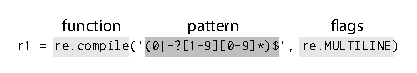
\includegraphics[width=\columnwidth]{illustrations/exampleUsage.eps}
%\vspace{-12pt}
%\caption{Example Python regex library invocation (credit: Chapman and Stolee~\cite{chapman2016})}
%\vspace{-6pt}
%\label{fig:exampleUsage}
%\end{figure}


\begin{table*}[ht]
\begin{small}\begin{center}
\caption{How frequently is each alternative expression style used?}
\label{table:nodeCount}
\begin{tabular}
{lll@{}rrrr}
name & description & example & nPatterns & \% patterns & nProjects & \% projects \\
\toprule[0.16em]
C1 & char class using ranges & \begin{minipage}{1.5in}\begin{verbatim}
'^[1-9][0-9]*$'\end{verbatim}\end{minipage}
 & 2,479 & 18.2\% & 810 & 52.5\%\\
C2 & char class explicitly listing all chars & \begin{minipage}{1.5in}\begin{verbatim}
'[aeiouy]'\end{verbatim}\end{minipage}
 & 1,283 & 9.4\% & 551 & 35.7\%\\
C3 & any negated char class & \begin{minipage}{1.5in}\begin{verbatim}
'[^A-Za-z0-9.]+'\end{verbatim}\end{minipage}
 & 1,935 & 14.2\% & 776 & 50.3\%\\
C4 & char class using defaults & \begin{minipage}{1.5in}\begin{verbatim}
'[-+\d.]'\end{verbatim}\end{minipage}
 & 840 & 6.2\% & 414 & 26.8\%\\
C5 & an OR of length-one sub-patterns & \begin{minipage}{1.5in}\begin{verbatim}
'(@|<|>|-|!)'\end{verbatim}\end{minipage}
 & 245 & 1.8\% & 239 & 15.5\%\\
\midrule
D1 & curly brace repetition like \{M,N\} with M<N & \begin{minipage}{1.5in}\begin{verbatim}
'^x{1,4}$'\end{verbatim}\end{minipage}
 & 367 & 2.7\% & 242 & 15.7\%\\
D2 & zero-or-one repetition using question mark & \begin{minipage}{1.5in}\begin{verbatim}
'^http(s)?://'\end{verbatim}\end{minipage}
 & 1,871 & 13.8\% & 646 & 41.8\%\\
D3 & repetition expressed using an OR & \begin{minipage}{1.5in}\begin{verbatim}
'^(Q|QQ)\<(.+)\>$'\end{verbatim}\end{minipage}
 & 10 & .1\% & 27 & 1.7\%\\
\midrule
T1 & no HEX, OCT or char-class-wrapped literals & \begin{minipage}{1.5in}\begin{verbatim}
'get_tag'\end{verbatim}\end{minipage}
 & 12,482 & 91.8\% & 1,485 & 96.2\%\\
T2 & has HEX literal like \verb!\xF5! & \begin{minipage}{1.5in}\begin{verbatim}
'[\x80-\xff]'\end{verbatim}\end{minipage}
 & 479 & 3.5\% & 243 & 15.7\%\\
T3 & has char-class-wrapped literals like [\$] & \begin{minipage}{1.5in}\begin{verbatim}
'[$][{]\d+:([^}]+)[}]'\end{verbatim}\end{minipage}
 & 307 & 2.3\% & 268 & 17.4\%\\
T4 & has OCT literal like \verb!\0177! & \begin{minipage}{1.5in}\begin{verbatim}
'[\041-\176]+:$'\end{verbatim}\end{minipage}
 & 14 & .1\% & 37 & 2.4\%\\
\midrule
L1 & curly brace repetition like \{M,\} & \begin{minipage}{1.5in}\begin{verbatim}
'(DN)[0-9]{4,}'\end{verbatim}\end{minipage}
 & 91 & .7\% & 166 & 10.8\%\\
L2 & zero-or-more repetition using kleene star & \begin{minipage}{1.5in}\begin{verbatim}
'\s*(#.*)?$'\end{verbatim}\end{minipage}
 & 6,017 & 44.3\% & 1,097 & 71.0\%\\
L3 & one-or-more repetition using plus & \begin{minipage}{1.5in}\begin{verbatim}
'[A-Z][a-z]+'\end{verbatim}\end{minipage}
 & 6,003 & 44.1\% & 1,207 & 78.2\%\\
\midrule
S1 & curly brace repetition like \{M\} & \begin{minipage}{1.5in}\begin{verbatim}
'^[a-f0-9]{40}$'\end{verbatim}\end{minipage}
 & 581 & 4.3\% & 340 & 22.0\%\\
S2 & explicit sequential repetition & \begin{minipage}{1.5in}\begin{verbatim}
'ff:ff:ff:ff:ff:ff'\end{verbatim}\end{minipage}
 & 3,378 & 24.8\% & 861 & 55.8\%\\
S3 & curly brace repetition like \{M,M\} & \begin{minipage}{1.5in}\begin{verbatim}
'U[\dA-F]{5,5}'\end{verbatim}\end{minipage}
 & 27 & .2\% & 32 & 2.1\%
 \\
\bottomrule[0.13em]
\end{tabular}
\end{center}\end{small}\end{table*}



\subsubsection{Features and Pattern}
%The presence of a feature is not always enough to determine membership.
%However, the presence of a feature and properties of the pattern can determine membership.
Identifying D3 requires an OR containing at least two entries with a sequence present in one entry repeated N times and the same sequence present in another entry repeated N+1 times. We first looked for a sequence of N repeating groups with an OR-bar (i.e., \verb!|!) next to them on a side. This produced a list of 113 candidates which we narrowed down manually to 10 actual members.


T2 requires a literal with a hex structure. %that matches the regex \verb!(\\x[a-f0-9A-F]{2})! which reliably identifies hex codes within a pattern.
T4 requires a literal with a %and must match the regex \verb!((\\0\d*)|(\\\d{3}))! which is specific to
Python-style octal structure. %, requiring either exactly three digits after a slash, or a zero and some other digits after a slash. One false positive was identified, which was actually the lower end of a hex range using the literal \verb!\0!.
T3 requires that a single literal character is wrapped in a custom character class (a member of T3 is always a member of C2).
T1 requires that no characters are wrapped in brackets or are hex or octal characters, which matches over 91\% of the patterns analyzed.

\subsubsection{Token Stream }
%The rest of the representations were identified by representing the regex patterns as a sequence of tokens.
S2 requires a repeated element. This element could be a character class, a literal, or a collection of things encapsulated in parentheses; rather than a parser, we used a token stream to identify it.
C1 requires that a non-negative character class contains a range.
C2 requires that there exists a custom character class that does not use ranges or defaults.
C4 requires the presence of a default character class within a custom character class.
%, specifically, \verb!\d!, \verb!\D!, \verb!\w!, \verb!\W!, \verb!\s!, \verb!\S! and \verb!.!.
C5 requires an OR of length-one sequences (literal characters or any character class).


\subsection{Results}
Table~\ref{table:nodeCount} presents the results.
% frequencies with which each representation appears in a regex pattern and in a project scraped from GitHub.
 \emph{Node} references Figure~\ref{fig:refactoringTree}, \emph{description} briefly describes the representation, \emph{example} provides a regex from the corpus. \emph{nPatterns} counts the patterns that belong to the representation, followed by the percent of patterns out of 13,597.
 \emph{nProjects} counts the projects that contain a regex belonging to the representation,
followed by the percentage of projects out of 1,544.
%The project support is used to show pervasiveness across the whole corpus.
For example, D1 appears in 346 (2.5\%) of the patterns but only 234 (15.2\%) of the projects.
 In contrast, T3 appears in 39 \emph{fewer} patterns but 34 \emph{more} projects, indicating that D1 is more concentrated in a few projects and T3 is more widespread across projects.

The pattern frequency is our guide for setting the community standards.
For example, since C1 is more prevalent than C2 in both patterns and projects, we could say that C2 is smelly since it could better conform to community standards if expressed as C1.
%Based on patterns alone, the winning representations per equivalence class are C1, D2, T1, L2, and S2. With one exception, these are the same for recommendations based on projects; L3 appears in more projects than L2, so it is unclear which is smelly.

%Our analysis simply suggests smells. %a direction for a refactoring (in this case, from C4 to C1).
%Section~\ref{sec:rq3} explores these results more deeply.

%Table~\ref{summaryResults} presents these recommendations for each pair of representations within each equivalence class. The \emph{Comm} column is populated based on the findings of \emph{RQ1}. The findings for \emph{RQ2} and \emph{RQ3} are in the \emph{Match} and \emph{Compose} columns, respectively.

\subsection{Summary}
Based on patterns, the winning representations per equivalence class are C1, D2, T1, L2, and S2. With one exception, these are the same project-based recommendations; L3 appears in more projects than L2, so it is unclear which is smelly.



\section{Understandability Study (RQ1)}
\label{sec:rq1}
This study presents  programmers with regexes and asks comprehension questions. By comparing the understandability of semantically equivalent regexes that match the same language but have different syntactic representations, we aim to identify understandability code smells.
This study was  implemented on Amazon's Mechanical Turk with 180 participants. A total of 35 pairs of regex were evaluated. Each regex pattern was evaluated by 30 participants.
%The patterns used were designed to belong to various representations in Figure~\ref{fig:refactoringTree}.







\subsection{Metrics}
\label{sec:understadningmetric}
 We measure the understandability of regexes using two complementary metrics, \emph{matching} and \emph{compostition}. These are referred to as the \emph{comprehension metrics}. 
For a deeper look at the data to gain a better understanding of factors that impact accuracy, we also compute \emph{regex length} and \emph{DFA size} for each regex. 


\textbf{Matching:}
 Given a pattern and a set of strings, a participant determines by inspection which strings will be matched by the pattern. There are four possible responses for each string, \emph{matches}, \emph{not a match}, \emph{unsure}, or blank. An example from our study is shown in Figure~\ref{fig:exampleQuestion}.

 The percentage of correct responses, disregarding blanks and unsure responses, is the matching score.
 For example, consider regex pattern \verb!`RR*'!, tge five strings shown in Table~\ref{matchingmetric}, and the responses from four participants in the \emph{P1}, \emph{P2}, \emph{P3} and \emph{P4} columns.
 The {\em Oracle} indicates  the first three strings match and the last two do not. \emph{P1} answers correctly for the first three strings and the fifth, but incorrectly on the fourth, so the matching score is $4/5 = 0.80$. \emph{P2} incorrectly thinks that the second string is not a match, so the score is also $4/5 = 0.80$.  \emph{P3} marks `unsure' for the third string and so the total number of attempted matching questions is 4. \emph{P3} is incorrect about the second and fourth string, so they score $2/4 = 0.50$.  For \emph{P4}, we only have data for the first and second strings, since the other three are blank.  \emph{P4} marks `unsure' for the second string so only one matching question has been attempted;  the matching score is $1/1 = 1.00$.

Blanks were incorporated into the metric because questions were occasionally left blank in the study. Unsure responses were provided as an option so not to bias the  results through blind guessing. These situations did not occur very frequently.
%Only 1.1\% of the responses were left blank and only 3.8\% of the responses were marked as unsure.  %We refer to a response with all blank or unsure responses as an `NA'.
Out of 1800 questions (180 participants * 10 questions each), only 1.8\%(32) were impacted by a blank or unsure response (never more than four out of 30 responses per pattern).


\begin{figure}[tb]
\centering
%\includegraphics[width=0.75\columnwidth]{illustrations/ExampleQuestion}
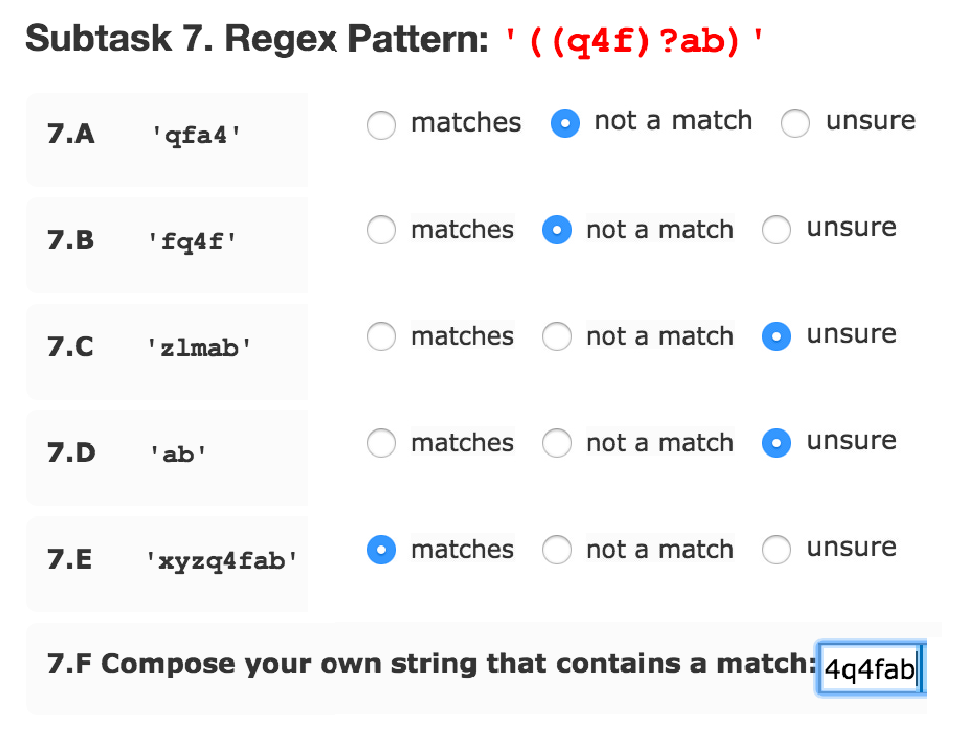
\includegraphics[width=0.75\columnwidth]{illustrations/exampleQuestion.eps}
\vspace{-12pt}
\caption{Questions from one pattern in one HIT}
\vspace{-6pt}
\label{fig:exampleQuestion}
\end{figure}



\begin{table} [t]
\caption{Matching metric example \label{matchingmetric}}
\begin{center}
%\begin{small}
\begin{tabular} {|cl | c c c c c|} \hline
\textbf{String} & \verb!`RR*'! & \textbf{Oracle} & \textbf{P1} & \textbf{P2} & \textbf{P3}& \textbf{P4}\\ \hline
1 & ``ARROW"    & \checkmark    & \checkmark    & \checkmark    & \checkmark    & \checkmark \\
2 & ``qRs"      & \checkmark    & \checkmark    & \xmark        & \xmark        & ?\\
3 & ``R0R"      & \checkmark    & \checkmark    & \checkmark    & ?             & -\\
4 & ``qrs"      & \xmark        & \checkmark    & \xmark        & \checkmark    & -\\
5 & ``98"       & \xmark        & \xmark        & \xmark        & \xmark        & -\\
\hline
  & Score       & 1.00          & 0.80          & 0.80          & 0.50          & 1.00\\ \hline
%\multicolumn{7}{l}{}\\
\multicolumn{7}{l}{\checkmark = match, \xmark = not a match, ? = unsure, -- = left blank}\\
\end{tabular}
%\end{small}
\end{center}
\vspace{-6pt}
\vspace{-6pt}
\end{table}



\textbf{Composition:}
Given a pattern, a participant composes a string they think it matches (question 7.F in Figure~\ref{fig:exampleQuestion}). If the participant is accurate, a composition score is 1, otherwise 0.  For example, given the pattern \verb!(q4fab|ab)! from our study, the string, ``xyzq4fab" matches  and gets a score of 1, but the string, ``acb" does not match and gets  a score of 0.

To determine a match, each pattern was compiled using the \emph{java.util.regex} library. A \emph{java.util.regex.Matcher} \verb!m! object was created for each composed string using the compiled pattern.  If \verb!m.find()! returned true, then that composed string was a match and scored 1, otherwise it scored 0.

\textbf{Regex Length:} 
Given a pattern, the regex length is computed by \todo{how was this done?}

\textbf{DFA Size:} 
To compute DFA size, we run both \textit{brics}~\cite{brics} and \textit{Rex}~\cite{rex} on each regex in order to get the minimal DFA. We note that \textit{brics} always shows the minimal DFAs but its syntax is very restricted in language coverage~\cite{chapman2016} while \textit{Rex} accepts most regular expression features, but does not guarantee a minimal DFA (although, as it turns out, most are minimal). %Although most of the DFAs generated by \textit{Rex} are minimal but they are not guaranteed to be minimal. 
For the regexes that are accepted by both \textit{brics} and \textit{Rex}, we chose the size of DFA generated from \textit{brics}. For the regexes only accepted by \textit{Rex}, we examined the generated DFAs manually and made minor changes to make sure we use the minimal one.



\subsection{Design}
%\todoNow{needs to be updated with respect to no C1,T1 nodes}
We implemented this study on  Amazon's Mechanical Turk (MTurk),  a crowdsourcing platform where requesters create human intelligence tasks (HITs) for completion by workers.
%Each HIT is designed to be completed in a fixed amount of time and workers are compensated with money if their work is satisfactory. Requesters can screen workers by requiring each to complete a qualification test prior to completing any HITs.

\subsubsection{Worker Qualification}
Workers qualified to participate  by answering questions regarding some basics of regex knowledge. These questions were multiple-choice and asked the worker to analyze the following patterns: \verb!a+!, \verb!(r|z)!, \verb!\d!, \verb!q*!, and \verb![p-s]!. To pass the qualification test, workers had to answer four of the five questions correctly.

\subsubsection{Tasks}
Using the patterns in the corpus as a guide, we created 60 regex patterns that were grouped into 26 semantic equivalence groups.
 There were 18 groups with two regexes that target various edges in the equivalence classes.
The other eight semantic groups had three regexes each, forming 42 total pairs.
These semantic groups were intended to explore edges in the equivalence classes. In this way, we can draw conclusions by comparing between representations since the regexes evaluated were semantically equivalent.

To form the semantic groups, we took a regex from the corpus, matched it to a representation in Figure~\ref{fig:refactoringTree}, trimmed it down so it contained little more than just the feature of interest, and then created other regexes that are semantically equivalent but belong to other nodes in the equivalence class. For example, a semantic group with regexes \verb!((q4f){0,1}ab!, \verb!((q4f)?ab)!, and \verb!(q4fab|ab)! belong to D1, D2, and D3, respectively.
A  group with regexes \verb!([0-9]+)\.([0-9]+)! and  \verb!(\d+)\.(\d+)! is intended to evaluate the edge between C1 and C4.
We note that if we only used regexes from the corpus, we would have had regexes with different semantics at each node, or with additional language features, which would make the comparisons of the targeted features  difficult.




%Using the patterns in the corpus as a guide, we created six metagroups containing three pairs of patterns focusing on:
%\begin{itemize}
%\item S1 vs S2
%\item the digit default character class vs C1
%\item the word default character class vs C1
%\item negated digits and words vs C3, whitespace vs C2
%\item additional vs kleene repetition
%\item wrapping vs escaping literal characters
%\end{itemize}
%and four metagroups containing two triplets of patterns focusing on
%\begin{itemize}
%\item octal vs hex vs literal
%\item D1 vs D2 vs D3
%\item C1 vs C2 vs C5
%\item octal vs literal and C2 vs C5
%\end{itemize}
%
%Each of these 10 metagroups contains 6 strings, resulting in a total of 60 regex patterns.  These patterns are logically partitioned into 26 semantic equivalence groups (18 from pairs, 8 from triples).


\begin{table}[t]
\centering
\caption{3-factor ANOVA results with accuracy as the dependent variable, considering representation, DFA size, and regex length as independent variables}
\begin{tabular}{@{}l@{}rrrrl@{}}
  \hline
 & Df & Sum Sq & Mean Sq & F value & Pr($>$F) \\ 
  \hline
dfa\_size              & 1 & 1.47 & 1.47 & 29.05 & 0.0000*** \\ 
  str\_len               & 1 & 0.61 & 0.61 & 12.09 & 0.0005*** \\ 
  rep                  & 15 & 6.04 & 0.40 & 7.97 & 0.0000*** \\ 
  dfa\_size:str\_len      & 1 & 0.20 & 0.20 & 3.98 & 0.0461* \\ 
  dfa\_size:prep         & 14 & 1.95 & 0.14 & 2.76 & 0.0005*** \\ 
  str\_len:prep          & 10 & 1.78 & 0.18 & 3.52 & 0.0001*** \\ 
  dfa\_size:str\_len:prep & 3 & 0.66 & 0.22 & 4.36 & 0.0045** \\ 
  Residuals             & 1722 & 87.03 & 0.05 &  &  \\ 
   \hline
\end{tabular}

\vspace{3pt}
.$\alpha = 0.10$ \hspace{3pt} *$\alpha=0.05$ \hspace{3pt} **$\alpha=0.01$ \hspace{3pt} ***$\alpha=0.001$
\label{table:anova}
\end{table}

For each of the 26 semantic groups, we created five strings for the study, where at least one matched and at least one did not match. These were used to compute the matching metric.

Once all the patterns and matching strings were collected, we created tasks for the MTurk participants as follows:
randomly select a pattern from 10 of the 26 semantic groups. Randomize the order of these 10 patterns, as well as the order of the matching strings for each pattern. After adding a question asking the participant to compose a string that each pattern matches, this creates one task on MTurk, such as the example in Figure~\ref{fig:exampleQuestion}.   This process was completed until each of the 60 regexes appeared in 30 HITs, resulting in a total of 180 total unique HITs.
%An example of a single regex pattern, the five matching strings and the space for composing a string is shown in

\begin{table*}\begin{small}\begin{center}\caption{Averaged Info About Edges}\label{table:testedEdgesTable}\begin{tabular}
{llccccccc}
index & edge & nExp & acc1 & acc2 & cmp1 & cmp2 & Pacc & Pcmp \\
\toprule[0.16em]
E1 & C1 -- C2 & 2 & 0.94 & 0.90 & 28.0 & 27.0 & 0.268800 & 0.802400\\
E2 & C1 -- C2, T2  -- T1 & 2 & 0.84 & 0.86 & 19.5 & 27.5 & 0.751200 & 0.031185\\
E3 & C1 -- C2,T4->T1 & 2 & 0.81 & 0.86 & 15.5 & 27.5 & 0.609700 & 0.022661\\
E4 & C1->C4 & 5 & 0.76 & 0.76 & 24.2 & 23.8 & 0.555860 & 0.500942\\
E5 & C1->C5 & 5 & 0.90 & 0.88 & 27.0 & 27.2 & 0.472560 & 0.551300\\
E6 & C2->C4 & 1 & 0.83 & 0.92 & 18.0 & 20.0 & 0.075020 & 0.788800\\
E7 & C2->C5 & 4 & 0.85 & 0.86 & 26.5 & 28.5 & 0.282075 & 0.598075\\
E8 & C2->C5,T4->T1 & 2 & 0.60 & 0.82 & 11.0 & 29.0 & 0.048688 & 0.000015\\
E9 & D1->D2 & 2 & 0.84 & 0.78 & 28.0 & 26.5 & 0.306450 & 0.598350\\
E10 & D1->D3 & 2 & 0.84 & 0.87 & 28.0 & 29.0 & 0.526250 & 0.802400\\
E11 & D2->D3 & 2 & 0.78 & 0.87 & 26.5 & 29.0 & 0.155290 & 0.598350\\
E12 & L2->L3 & 3 & 0.86 & 0.91 & 27.3 & 29.3 & 0.230233 & 0.751533\\
E13 & S1->S2 & 3 & 0.86 & 0.85 & 27.0 & 26.3 & 0.420767 & 1.000000\\
E14 & T1->T3 & 3 & 0.88 & 0.86 & 21.7 & 22.7 & 0.177233 & 0.697267\\
E15 & T1->T4 & 2 & 0.80 & 0.60 & 26.0 & 11.0 & 0.049250 & 0.002759\\
E16 & T2->T4 & 2 & 0.84 & 0.81 & 19.5 & 15.5 & 0.519000 & 0.535040\\
\bottomrule[0.13em]\end{tabular}\end{center}\end{small}\end{table*}


\subsubsection{Implementation}
Workers were paid \$3.00 for successfully completing a HIT, and were only allowed to complete  one HIT.  The average completion time for accepted HITs was 682 seconds (11 mins, 22 secs).
%A total of 241 HITs were submitted - of those 55 were rejected.
%, and 6 duplicates were ignored, always using the first accepted submission so as to obtain a value for each of the 180 distinct tasks.
A total of 54 HITs were rejected: 48 had too many blank responses, four were double-submissions by the same worker, one  did not answer the composition questions, and one was missing data for 3 questions.  Rejected HITs were returned to MTurk to be completed by others.


%
%
%
%\begin{figure}[tp]
%\begin{small}
%\fbox{\parbox{\columnwidth}{
%\begin{enumerate}
%\item
%\begin{tabular} {lrr}
%\textbf{What is your gender?} & \textbf{n} & \textbf{\%}\\ \hline
%Male & 149 & 83\%\\
%Female & 27& 15\%\\
%Prefer not to say & 4& 2\%
%\end{tabular}
%\item \textbf{What is your age?} \\
%$\mu = 31$, $\sigma = 9.3$
%
%\item
%
%\begin{tabular} {l |rr}
%\textbf{Education Level?} & \textbf{n} & \textbf{\%}\\ \hline
%High School & 5 & 3\%\\
%Some college, no degree & 46 & 26\%\\
% Associates degree & 14 & 8\%\\
%Bachelors degree & 78 & 43\%\\
%Graduate degree & 37 & 21\%\\
%\end{tabular}
%\item
%\begin{tabular} {lrr}
%\textbf{Familiarity with regexes?} & \textbf{n} & \textbf{\%}\\ \hline
%Not familiar at all & 5 & 3\%\\
%Somewhat not familiar & 16 & 9\%\\
%Not sure & 2 & 1\%\\
%Somewhat familiar & 121 & 67\%\\
%Very familiar & 36 & 20\%\\
%\end{tabular}
%\item \textbf{How many regexes do you compose each year?} \\
%$\mu = 67$, $\sigma = 173$
%\item \textbf{How many regexes (not written by you) do you read each year?} \\
%$\mu = 116$, $\sigma = 275$
%%\item In what contexts do you use regexes? \\
%\end{enumerate}
%}}
%\caption{Participant Profiles, $n=180$ \todoLast{can remove this for space} \label{participantprofile}}
%\end{small}
%\end{figure}
%


\subsubsection{Participants}

In total, there were 180 participants.
A majority were male (83\%). % with an average age of 31.
Most had
at least an Associates degree (72\%), were at least somewhat familiar with regexes (87\%), and have prior programming experience (84\%).
%On average,
%participants compose 67 regexes per year with a range from 0 to 1000.
%Participants read more regexes than they write with an average of 116 and a range from 0 to 2000.
%Figure~\ref{participantprofile} summarizes the self-reported participant characteristics from the qualification survey.


%\todoNow{in study section present choices about pairwise vs random selection for nodes.}


\subsection{Analysis}
For each of the 180 HITs, we computed a matching and composition score for each of the 10 regexes, using the metrics described in Section~\ref{sec:understadningmetric}. This allowed us to compute and then average 26-30 values for each metric  for each of the 60 regexes (fewer than 30 values were used if all the responses in a matching question were a combination of blanks and unsure). %Next, we computed average scores for matching and composition per regex.
%\todoLast{Mentioning NAs here?}


%Each regex was a member of one of 26 groupings of equivalent regexes.
%These groupings allow pairwise comparisons of the metrics values to determine which representation of the regex was most understandable and the direction of a refactoring for understandability.
Of the original 42 pairs, we report scores for only 41 pairs. Due to a design flaw, the regexes evaluated, \verb!\..*! and \verb!\.+!. were not semantically equivalent (the former is missing an escape and should be \verb!\.\.*!), so this was omitted from the data. In the end, we analyzed 58 regexes that cover  17 edges from Figure~\ref{fig:refactoringTree}.

To gain a better understanding of why some regexes may be more understandable than others, we also look at the impact of the representation from Figure~\ref{fig:refactoringTree}, regex  length, and DFA size on accuracy. 
Note that  we retain all 60 regexes for this analysis as we are looking at the properties of regexes individually. 
We conduct a three-factor analysis of variance (ANOVA) with accuracy as the dependent variable.
We also conduct the correlation analysis between each factors and the accuracy. 
We use Spearman's Rank-Order Correlation because we have no priori knowledge about the distributions of the factors. 
Since  the regex representations are categorical data, these are excluded from the correlation analysis. 



\subsection{Results}
Table~\ref{table:anova} shows that DFA size, string length,  representations, and their interactions all significantly affect the accuracy. As a result, we present our results for the matching and composition metrics using each of the 41 pairs of regexes separately, rather than in aggregate (Table~\ref{table:testedEdgesTable}, discussed later in this section). 



%\textcolor{red}{Todo: update Table and its description, add annova and correlation analysis about representation, dfa size, and string length}

For the comprehension metrics, Table~\ref{table:testedEdgesTable} presents the results.
Each row represents a {\em Pair} of regex evaluated by study participants.
The representations for the regexes per Figure~\ref{fig:refactoringTree} are shown in the {\em Edge} column, which is how the table is sorted. 
The {\em Regex 1} and {\em Regex 2} columns identify the regexes used in the study, mapping to the first and second representations in the {\em Edge}, respectively. 
{\em Acc1} is the average accuracy for {\em Regex 1} and {\em Acc2} is the average accuracy for {\em Regex 2}. 
Using the Mann-Whitney test of means, the {\em sig} column following tests if there is a significant difference between the accuracies. 
The {\em Comp1} column presents the percentage of the string responses for that were in fact correctly matched by {\em Regex 1}. {\em Comp2} presents the same information, except for {\em Regex 2}. 
The following {\em sig} column uses a test of two proportions to identify if the percentage of the participants who correctly composed a string for Regex 1 is significantly different than the percentage who correctly composed a string for {Regex 2}. 
If both comprehension metrics indicated a preferred representation, that representation is bolded in the \emph{Edge} column. If no preference is obvious, neither representation is bolded. 

%, \emph{Nodes} lists the representations, \emph{Pairs} shows the number of comparisons, \emph{Example Preferred Regex} shows a regex from the preferred node (bolded in \emph{Pairs} column), \emph{Match1} and \emph{Match2} give the matching scores for the first and second representations, respectively, and $H_0: \mu_{match1} = \mu_{match2}$ uses the Mann-Whitney test of means to compare the matching scores, and presents the p-values. The last three columns list the average composition scores for the representations and the composition p-value.

For example, consider row 16 in Table~\ref{table:testedEdgesTable}.
One pair of regexes was \verb!([}{])! and \verb!(\{|\})! in C4 and C5, respectively, with average matching scores of 0.79  and 0.70 and average composition scores of 50.00\%  and 86.67\%, respectively.
The difference between the composition scores is significant at $\alpha = 0.01$, yet the difference between the accuracies is not. 
In fact, the representation C5 was more understandable in that participants could more effectively compose a string that it would match, but C4 is more understandable in that participants could more easily determine which of a set of strings would be matched by C4. Thus, neither representation is bolded since there is a conflict. 
%Thus, the community found \verb!R+! from L3 more understandable.
%This is not the only regex pair in E5, however, The other is \verb!zaa*! and \verb!za+!. %, and regexes pair \verb!\..*! and \verb!\.+'!.
%In aggregate, considering both regex pairs, the overall matching average for the regexes belonging to L2 was 0.86 and 0.91 for L3.
%The overall composition score for L2 was 0.97 and 1.00 for L3.
%The community found L3 to be more understandable than L2, from the perspective of both metrics, suggesting that L2 is generally smelly, though the differences are not significant.



\begin{figure}[tb]
\centering
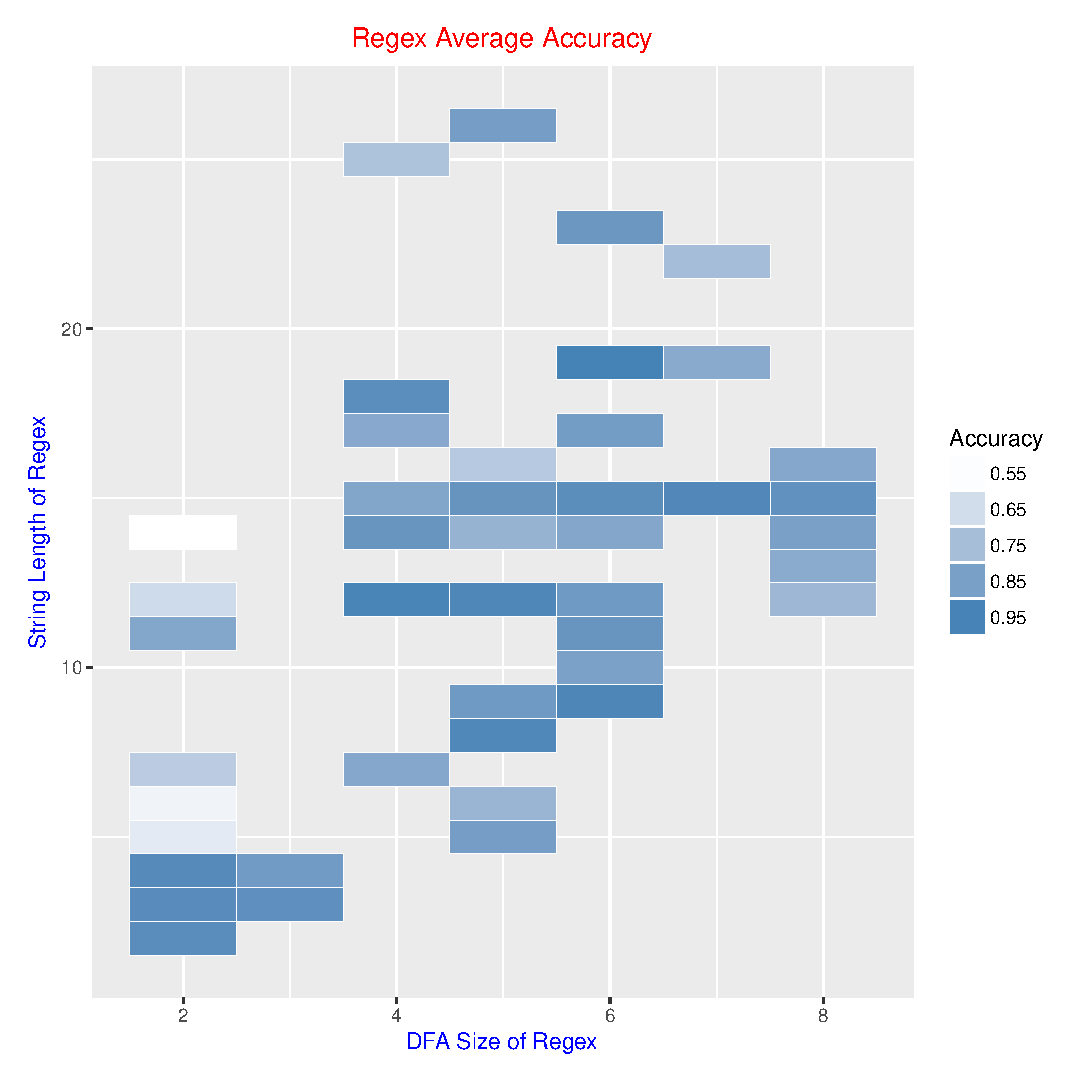
\includegraphics[width=0.75\columnwidth]{graphs/heatmap_avgAccur.eps}
\vspace{-12pt}
\caption{Heatmap for impacts of DFA size and regex string length on accuracy}
\vspace{-6pt}
\label{fig:heatmap}
\end{figure}

%60 strings
%42 comparisons
%18@2, 8@3
%
%M6R1 ? group 3, 3 comparisons
%- 1 comparisons
%- 0 strings
%
%M3R0 ? group 3, 3 comparisons
%- 1 comparisons
%- 0 strings
%
%M3R1 ? group 3, 3 comparisons
%- 2 comparisons
%- 1 string
%
%M3R0 ? group 3, 3 comparisons
%- 2 comparisons
%- 1 string
%
%58 strings
%36 comparisons


%Although we performed 42 pairwise comparisons,

%\subsection{Results}
% In E1 through E4, there is a statistically significant difference between the representations for at least one of the metrics with $\alpha = 0.10$.  These represent the strongest evidence for code smells, suggesting that T4, D2, and C2 are less understandable.
 
For pairs 16, 29, 34, and 36, the difference in composition is significant at $\alpha < 0.05$, indicating differences favoring C5 over C4, T1 over T2, and two favoring T1 over T4. 
For pairs 23, 37, and 38, the difference in accuracy is significant with $\alpha < 0.05$, indicating differences favoring D3 over D2 and two favoring T1 over T4. 
There appears to be a clear trend favoring T1 over T4. Interestingly, for pairs 16 and 29, while the differences in composition are significant, there is a conflict between the metrics. Further investigation is needed to understand in what circumstances the metrics are in conflict with one another. 


% and we can use that to further corroborate the understandability analysis.

%\begin{table*}
%\centering
%\caption{Average Unsure Responses Per Pattern By Node (fewer unsures on the left)}\label{table:unsureResults}
%\begin{tabular}{|| l || cccc || cccc || || cccc || cccc ||}
%                & \multicolumn{4}{c||}{>=Q0(0.67)}         & \multicolumn{4}{c||||}{>=Q1(1.25)}   & \multicolumn{4}{c||}{>=Q2(1.94)}    &  \multicolumn{4}{c||}{>=Q3(2.54)}  \\ \hline
%Node     & L3 & D3 & C2 & C1 & L2 & S2 & S1 & C4 & D1 & C5 & C3 & D2 & T1 & T3 & T2 & T4 \\
%% Number of Patterns - reversed & 4 & 2 & 3 & 3 & 2 & 2 & 4 & 2 & 9 & 3 & 3 & 3 & 8 & 5 & 2 & 3\\
%Unsure Responses Per Pattern & 0.7 & 1 & 1 & 1 & 1.3 & 1.7 & 1.7 & 1.9 & 2 & 2 & 2 & 2.5 & 2.7 & 2.7 & 5.5 & 8.5\\
%\end{tabular}
%\end{table*}
Recall that participants were able to select \emph{unsure} for whether a string is matched  by a pattern.
From a comprehension perspective, this indicates some level of confusion.
For each pattern, we counted the number of responses containing at least one unsure.
%We then grouped the patterns into their representation nodes and computed an average of unsures per pattern.
%A higher number may indicate difficulty in comprehending a pattern from that node.
Overall, the highest number of unsure responses came from T4 and T2, which have octal and hex representations of characters. The least number of unsure responses were in L3 and D3.
%, which are both shown to be understandable by looking at E2 and E3 in Table~\ref{table:testedEdgesTable}.
%These nodes and their average number of unsure responses are organized by quartile in Table~\ref{table:unsureResults}.
These results mirror the understandability analysis, as T4 and T2 are generally lower in comprehension, and L3 and D3 are generally higher.%, echoing that L3 and D3 are less smelly.
% for the LIT group (i.e., $\overrightarrow{T4 T1}$), the DBB group (i.e.,  $\overrightarrow{D2 D3}$), and the LWB group (i.e., $\overrightarrow{L2 L3}$) because the more understandable node has the least unsures of its group.
% The findings for D3 and D2 are contradictory, however, as  and further study is needed.
%  and the number of unsures may be too small to indicate anything, except for T2 and T4.  The one pattern from T4 that had the most unsures of any pattern (i.e., 10 out of 30) was \verb!`xyz[\0133-\0140]'!, so this may have been the least understandable pattern that we tested.

While the ANOVA indicates that variance in accuracy is due to all three factors, representation, DFA size, and regex length, it is not entirely clear why. 
Between regex length and accuracy, Spearman's  $\rho=-0.025$, indicating  a weak negative relationship. 
For DFA size the accuracy,   the correlation is weak and positive $\rho=0.07$. At first, this result may seem counter-intuitive, but considering that larger DFAs may represent more constrained regex languages (i.e., languages that accept fewer strings), these may be easier to understand. %the regular language with a relatively small scope and thus easier for people to recognize. 

Figure~\ref{fig:heatmap} is a heatmap showing the average accuracies of the 60 regexes along with their DFA size and string length. From the figure, we can see the color is darker towards the bottom and left, which confirms the correlation analysis results. \todo{I'm not convinced that the heatmap provides enough value to keep in the paper.}
We also note that since composition is either 1 or 0, we do not perform an ANOVA with composition as the dependent variable. \todo{is this the correct decision?}


%\todo{impact of size on matching, composition}





\section{Desirable Representations (RQ3)}
\label{sec:rq3}
To determine the overall trends in the data, we created and compared total orderings on the representations in each equivalence class with respect to the comprehension (RQ1) and community standards (RQ2) metrics.

\subsection{Analysis}
Total orderings were represented in directed graphs with representations as nodes and edge directions determined by the metrics: matching and composition of understandability; patterns and projects of community standards. The graphs for comprehension are based on Table~\ref{table:testedEdgesTable} and for community support are based on Table~\ref{table:nodeCount}. Within each graph, a topological sort created total orderings.


%The following sections describe the process for building and sorting the graphs.



%\subsubsection{Building the Graphs}
\textbf{Building the Graphs:}
In the community standards graph, a directed edge $\overrightarrow{C2 C1}$ is used when nPatterns(C1) $>$ nPatterns(C2) \emph{and} nProjects(C1) $>$ nProjects(C2).
When there is a conflict between nPatterns and nProjects, as is the case between L2 and L3,
%where L2 is found in more patterns and L3 is found in more projects,
an undirected edge $\overline{L2L3}$ is used. % as there is no winner based on the metrics.
%After considering all pairs of nodes in each equivalence class that also have an edge in Figure~\ref{fig:refactoringTree}, we create graphs,
For example, Figure~\ref{fig:graphsforanalysis} shows the graphs for the CCC group; Figure~\ref{fig:graphsforanalysis}b is based on community standards.

A similar process is used to build the graphs based on the comprehension metrics.
In Table~\ref{table:testedEdgesTable}, each row maps to an edge in the understandability graph.
If the matching and composition results both indicate a favorite (i.e., a bolded representation in the {\em Edge} column of Table~\ref{table:testedEdgesTable}), there is a directed edge. For example, in Pair~3, the matching and composition metrics for C3 are higher than C1, resulting in a directed $\overrightarrow{C1 C3}$ arrow. If one of the metrics is a tie, the other is used to break the tie; in Pair~2, the composition scores are the same but C1 is preferred based on matching, resulting in a $\overrightarrow{C2 C1}$. If there is a conflict between the metrics, an undirected edge is used, as is the case with Pair~14, resulting in $\overline{C3 C4}$.
An example is shown in Figure~\ref{fig:graphsforanalysis}a, which has 17 total edges, 14 of which are directed and three are undirected.

As a general rule, for both graphs, the higher the ratio of incoming edges to total edges, the less smelly the node.
%Nodes with fewer incoming edges are more smelly and nodes with more incoming edges are less smelly.
%Note that with the CCC group, there is no edge between C3 and C5 because there is no straightforward refactoring between those representations, as discussed in Section~\ref{sec:refactoring}.


\begin{figure}[tb]
\centering
%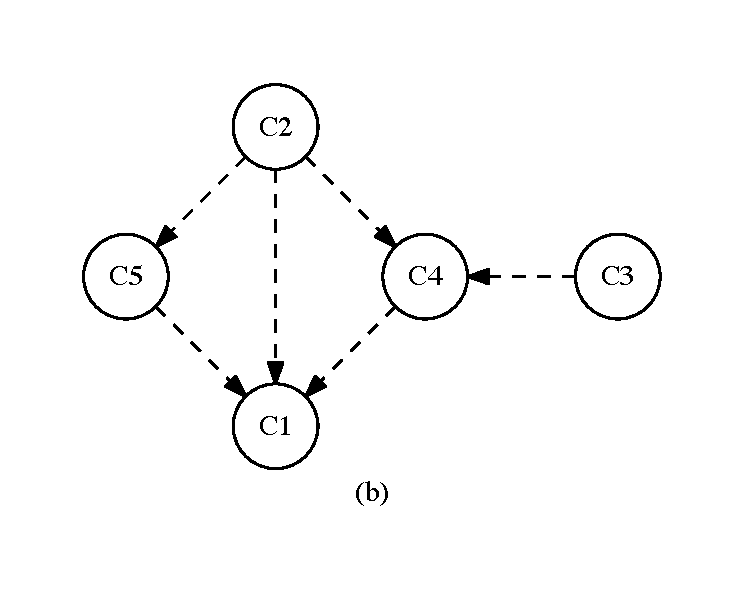
\includegraphics[width=0.57\columnwidth]{graphs/ccom.pdf}
%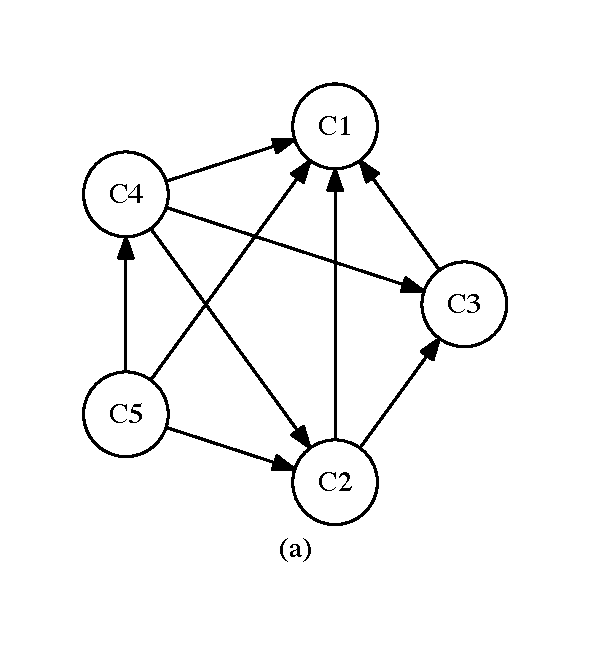
\includegraphics[width=0.40\columnwidth]{graphs/cart.pdf}
%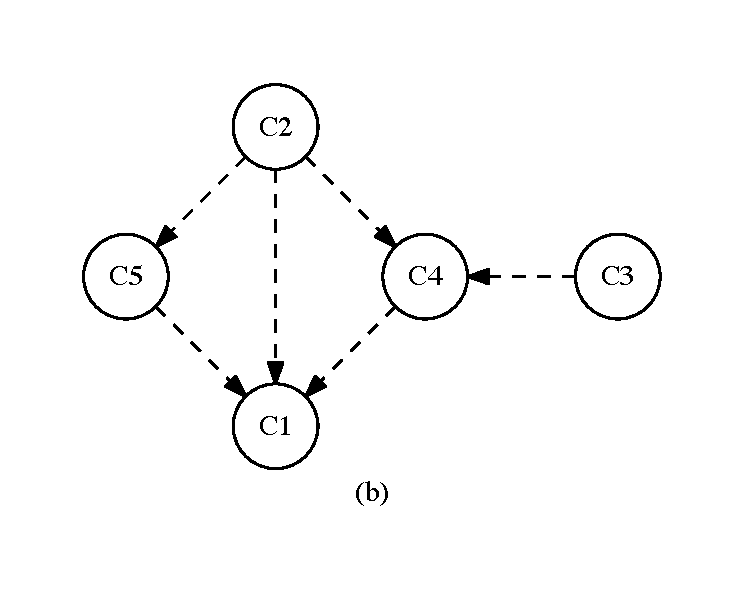
\includegraphics[width=0.35\columnwidth]{graphs/ccom.pdf}
%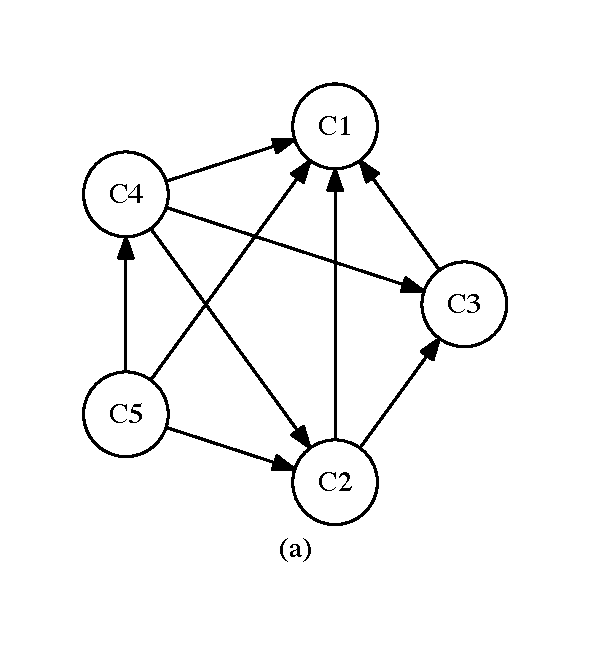
\includegraphics[width=0.35\columnwidth]{graphs/cart.pdf}
\includegraphics[width=0.35\columnwidth]{graphs/ccom.eps}
\includegraphics[width=0.35\columnwidth]{graphs/ccart.eps}
\vspace{-6pt}
\caption{Trend graphs for the CCC equivalence graph: (a) represent the comprehension analysis (RQ1) and (b) represent the artifact analysis (RQ2)}
\vspace{-6pt}
\vspace{-3pt}
\label{fig:graphsforanalysis}
\end{figure}
%\begin{table}
%\centering
%\caption{Topological Sorting, with the left-most position being highest \label{topologicalResults}}
%\begin{footnotesize}
%\begin{tabular}{| l | l | l | l | l | l |} \hline
%				& CCC			& DBB 		& LBW & SNG & LIT \\ \hline
%U 			& C1 C5 C4 C2 C3 	& D3 D1 D2 	& L3 L2		& S2 S1		& T1 T2 T4 T3 \\
%C		& C1 C3 C2 C4 C5 	& D2 D1 D3	&  L3 L2 L1 	& S2 S1 S3 	& T1 T3 T2 T4 \\
%\hline
%\end{tabular}
%\end{footnotesize}
%\end{table}






%In the understandability graph, we represent a directed edge $\overrightarrow{C2C1}$ when match(C1) $>$ match(C2) \emph{and} compose(C1) $>$ compose(C2). When there is a conflict between match and compose, as is the case with T1 and T3 where match(T1) is higher but compose(T3) is higher, an undirected edge $\overline{T1T3}$ is used. When one metric has a tie, as is the case with composition in E9, we use the other metric to determine $\overrightarrow{C5C1}$. An example understandability graph for the CCC is shown in Figure~\ref{fig:graphsforanalysis}b. Nodes with few incoming edges are less understandable (or were not evaluated in our study), and nodes with more incoming edges were more understandable.
%\footnote{When there are confounded representations, as is the case with E8, E4, and E5 which all use transformations from the CCC and the LIT equivalence classes, we omit those from the understandability graph. This makes sense since all use a transformation between T1 and T4 strongly favoring T1. }

%\subsubsection{Topological Sorting}
\textbf{Topological Sorting:}
Once the two graphs are built for each equivalence class type, within each graph, we sort the nodes to identify a (preferably unique) total ordering on the nodes. This ordering represents preferences from the perspective of the comprehension or community standards metrics.
%we apply a modified version of Kahn's topological sorting algorithm to obtain a total ordering.
%The first modification is to remove all undirected edges since Kahn's operates over a directed graph.
%To begin, any disconnected nodes are added to the end of the topologically sorted list $L$.
%In Kahn's algorithm, all nodes without incoming edges are added to a set $S$, which represents the order in which nodes are explored in the graph. For each $n$ node in $S$, all edges from $n$ are removed and $n$ is added to a list $L$. If there exists a node $m$ that has no incoming edges, it is added to $S$. In the end, $L$ is a topologically sorted list.
%\begin{algorithm}
% \caption{Modified Topological Sort}\label{topological}
% \begin{algorithmic}[1]
%\State  $L \gets$ []
%\State $S \gets$ []
%\State Remove all undirected edges (creates a DAG) \label{removeundir}
%\State Add all disconnected nodes to $L$ and remove from graph. If there is more than one, mark the tie. \label{markTie1}
%\State Add all nodes with no incoming edges to $S$. If there is more than one, mark the tie. \label{addnoincomingtos}
%\While {$S$ is non-empty} \label{beginwhile}
%	\State remove a node $n$ from $S$ \label{setn}
%	\State add $n$ to $L$  \label{addntoL}
%	\For {node $m$ such that $e$ is an edge $\overrightarrow{nm}$}
%		\State remove $e$
%		\If{$m$ has no incoming edges}
%			\State add $m$ to $S$ \label{addToS}
%		\EndIf
%	\EndFor
%	\State If multiple nodes were added to $S$ in this iteration, mark the tie \label{markTie2}
%	\State remove $n$ from graph
%\EndWhile
%\State For all ties in $L$, use a tiebreaker.
%  \end{algorithmic}
%\end{algorithm}

For each node $n$, we compute the ratio of $in\_deg(n) / deg(n)$ where $in\_deg(n)$ is the number of incoming edges to $n$, and $deg(n)$ is the total edges touching~$n$. For example, in Figure~\ref{fig:graphsforanalysis}a, $in\_deg(C5) = 2$ and $deg(C5) = 5$.
The higher the ratio (that is, the more incoming edges indicating preference), the higher the node appears in the sorted list. For example, with node C1 in Figure~\ref{fig:graphsforanalysis}a, the ratio is $7 / 10$ since C1 is involved in ten total comparisons and is favored in seven. The ratio for node C2 is $1 / 5$ as C2 is involved in five comparisons, is preferred in one, is strictly not preferred in three, and has one with no preference, represented as an undirected edge.

One challenge with this (and any topological sorting approach, such as Kahn's algorithm), is that the total ordering is not necessarily unique and often multiple nodes have similar properties.
Thus, we mark ties in order to identify when a tiebreaker is needed.
% to enforce a total ordering on the nodes (though admittedly, it is not always unique).
%For example, on the understandability graph in Figure~\ref{fig:graphsforanalysis}, there is a tie between C3 and C2 since both have no incoming edges, so they are marked as a tie. Further, if C3 is added to $S$ first, when $n=C2$, both C5 and C4 are added to $S$, thus the tie between them is marked. In these cases, a tiebreaker is needed.
Breaking ties on the community standards graph involves choosing the representation that appears in a larger number of projects, as it is more widespread across the community.
Breaking ties in the understandability graph uses the RQ1 results. Based on Table~\ref{table:testedEdgesTable}, we compute the average metrics for each representation and select the winner.
%For example, C4 appears in E5, E12, and E13 with an overall average matching score of 0.81 and composition score of 24.3. C5 appears in E4 and E9 with an average matching of 0.87 and composition of 28.28. Thus, C5 is favored to C4 and appears higher in the sorting.

\begin{table}
\vspace{2mm}
\centering
\caption{Topological Sorting, with the left-most position being highest (non-smelly) and the right-most being most smelly \label{topologicalResults} }
%\vspace{-6pt}
\vspace{-3pt}
\begin{tabular}{| l | l | l |}  \hline
& Understandability & Community  \\ \hline
CCC & C1 C5 C3 C4 C2  &   C1 C3 C2 C4 C5  \\
DBB & D3 D1 D2  &   D2 D1 D3\\
 LBW & L3 L2	 &  L3 L2 L1 	\\
 SNG &  S2 S1 &  S2 S1 S3 \\
 LIT & T1 T3 T2 T4 & T1 T3 T2 T4 \\
\hline
\end{tabular}
\vspace{-6pt}
\vspace{-3pt}
%\vspace{-3pt}
\end{table}


\subsection{Results}
The total orderings on nodes for each graph are shown in Table~\ref{topologicalResults}. For example, given the graphs in Figure~\ref{fig:graphsforanalysis}a and Figure~\ref{fig:graphsforanalysis}b, the topological sorts are {\tt C1 C5 C3 C4 C2} and {\tt C1 C3 C2 C4 C5}, respectively.



Considering both topological sorts, there is a clear winner in each equivalence class except DBB. 
%, with the exception of DBB.
%That is, the node sorted highest in the topological sorts for both the community standards and understandability analyses are
This is C1 for CCC, L3 for LBW, S2 for SNG, and T1 for LIT.
%While the least-smelly representation is relatively clear, the smelliest representation varies.
%After the top rank, the second rank varies depending on the metric, however, h
While L3 is the winner for the LBW group, we note that L2 appears in slightly more patterns.
DBB is different as the orderings are completely reversed depending on the analysis. %, so the community standards favor D2 and understandability favors D3.
Further study is needed on this, as well as LBW and SNG since not all nodes were considered in the understandability analysis.

These results can guide regex design.
For example, to match numbers from one to 999, there are (at least) three options: $A$~=~{\tt [1-9]|[1-9][0-9]|[1-9][0-9][0-9]}, $B$~=~{\tt [1-9][0-9]?[0-9]?}, and $C$~=~{\tt [1-9][0-9]\{0,2\}}.
$A$ contains representations \{C1, D3, S2\}, $B$ contains \{C1,~D2\}, and $C$ contains \{C1, D1\}. % D3 and S2, B contains C1 and D2, and C contains C1 and D1.
According to Table~\ref{topologicalResults}, the sorting in understandability is \texttt{A\textgreater C\textgreater B} since \texttt{D3\textgreater D1\textgreater D2}. However, what we usually see in source code are B and C but not A. The reason might be that the representation of A takes more time to type, or may have a longer runtime performance.
In another example, we prefer {\tt \$[0-9]*.[0-9][0-9]} to {\tt \$[0-9]*.[0-9]\{2\}} in order to match dollar amounts. This is because S2 in the former regex is preferred to S1 in the latter regex, for all metrics.
%

\subsection{Summary}
Having a consistent and clear winner is evidence of a preference with respect to community standards and understandability, and thus provides guidance for potential refactoring.
This positive result, that the most popular representation in the corpus is also the most understandable, makes sense as people may be more likely to understand things that are familiar or well documented.




\begin{table}[t]
\caption{Summary of Refactoring Directions \label{summaryResults}}
\begin{center}
\begin{tabular}{|c@{ }c | c  l l @{}|} \hline
\multicolumn{2}{|c|}{\textbf{Pair}} & \textbf{Com} & \textbf{Match} & \textbf{Compose} \\ \hline \hline
C1 & C2 & $\Leftarrow$  & $\Leftarrow$ (E1) $\Rightarrow$ (E2,E3) & $\Leftarrow$ (E1) $\Rightarrow$ (E2,E3)\\
C1 & C3 & $\Leftarrow$ & & \\
\textbf{C1} & C4 & $\Leftarrow$ & $\equiv$ (E4) & $\Leftarrow$  (E4)\\
C1 & C5 & $\Leftarrow$ & $\Leftarrow$ (E5) & $\Rightarrow$ (E5) \\
C2 & C3 & $\Rightarrow$ & & \\
C2 & C4 & $\Leftarrow$ & $\Rightarrow$ (E6) & $\Rightarrow$ (E6)\\
C2 & C5 & $\Leftarrow$ & $\Rightarrow$ (E7,E8) & $\Rightarrow$ (E7,E8)\\
C3 & C4 & $\Leftarrow$ & & \\
C3 & C5 & $\Leftarrow$ & & \\
C4 & C5 & $\Leftarrow$ & & \\
\hline
D1 & D2 & $\Rightarrow$ & $\Leftarrow$ (E9)& $\Leftarrow$ (E9) \\
D1 & \textbf{D3} & $\Rightarrow$ & $\Rightarrow$ (E10)& $\Rightarrow$ (E10) \\
D2 & D3 & $\Leftarrow$ & $\Rightarrow$ (E11) & $\Rightarrow$ (E11) \\
\hline
L1 & L2 & $\Rightarrow$ & & \\
L1 & L3 & $\Leftarrow$ & & \\
L2 & L3 & $\Leftarrow$ & $\Rightarrow$ (E12) & $\Rightarrow$ (E12)  \\
\hline 
S1 & S2 & $\Rightarrow$ & $\Leftarrow$ (E13) & $\Leftarrow$ (E13) \\
S1 & S3 & $\Leftarrow$ & & \\
S2 & S3 & $\Leftarrow$ & & \\
\hline 
\textbf{T1} & T2 & $\Leftarrow$  & $\Leftarrow$ (E2)& $\Leftarrow$ (E2) \\
T1 & T3 & $\Leftarrow$ & $\Leftarrow$ (E14) & $\Rightarrow$ (E14)\\
\textbf{T1} & T4 & $\Leftarrow$ & $\Leftarrow$ (E3,E8,E15) & $\Leftarrow$ (E3,E8,E15)\\
T2 & T3 & $\Leftarrow$ & & \\
\textbf{T2} & T4 & $\Leftarrow$ & $\Leftarrow$ (E16) & $\Leftarrow$ (E16)\\
T3 & T4 & $\Leftarrow$ & & \\
\hline
%1 & 2 &  & & \\
%1 & 3 &  & & \\
%2 & 3 &  & & \\


\end{tabular}
\end{center}
\end{table}


\section{Results}
\label{sec:results}
Table~\ref{summaryResults} summarizes the results of the RQs.  \todoMid{This table does not show anything about significance... I wonder if we could do something like $\rightarrow$ for no significance (just based on averages) and $\Rightarrow$ for significance... just a thought. We could do a test of two proportions for the Com column. Some entries will be n/a for match and compose}

\begin{table*}[ht]
\begin{small}\begin{center}
\caption{How frequently is each alternative expression style used?}
\label{table:nodeCount}
\begin{tabular}
{lll@{}rrrr}
name & description & example & nPatterns & \% patterns & nProjects & \% projects \\
\toprule[0.16em]
C1 & char class using ranges & \begin{minipage}{1.5in}\begin{verbatim}
'^[1-9][0-9]*$'\end{verbatim}\end{minipage}
 & 2,479 & 18.2\% & 810 & 52.5\%\\
C2 & char class explicitly listing all chars & \begin{minipage}{1.5in}\begin{verbatim}
'[aeiouy]'\end{verbatim}\end{minipage}
 & 1,283 & 9.4\% & 551 & 35.7\%\\
C3 & any negated char class & \begin{minipage}{1.5in}\begin{verbatim}
'[^A-Za-z0-9.]+'\end{verbatim}\end{minipage}
 & 1,935 & 14.2\% & 776 & 50.3\%\\
C4 & char class using defaults & \begin{minipage}{1.5in}\begin{verbatim}
'[-+\d.]'\end{verbatim}\end{minipage}
 & 840 & 6.2\% & 414 & 26.8\%\\
C5 & an OR of length-one sub-patterns & \begin{minipage}{1.5in}\begin{verbatim}
'(@|<|>|-|!)'\end{verbatim}\end{minipage}
 & 245 & 1.8\% & 239 & 15.5\%\\
\midrule
D1 & curly brace repetition like \{M,N\} with M<N & \begin{minipage}{1.5in}\begin{verbatim}
'^x{1,4}$'\end{verbatim}\end{minipage}
 & 367 & 2.7\% & 242 & 15.7\%\\
D2 & zero-or-one repetition using question mark & \begin{minipage}{1.5in}\begin{verbatim}
'^http(s)?://'\end{verbatim}\end{minipage}
 & 1,871 & 13.8\% & 646 & 41.8\%\\
D3 & repetition expressed using an OR & \begin{minipage}{1.5in}\begin{verbatim}
'^(Q|QQ)\<(.+)\>$'\end{verbatim}\end{minipage}
 & 10 & .1\% & 27 & 1.7\%\\
\midrule
T1 & no HEX, OCT or char-class-wrapped literals & \begin{minipage}{1.5in}\begin{verbatim}
'get_tag'\end{verbatim}\end{minipage}
 & 12,482 & 91.8\% & 1,485 & 96.2\%\\
T2 & has HEX literal like \verb!\xF5! & \begin{minipage}{1.5in}\begin{verbatim}
'[\x80-\xff]'\end{verbatim}\end{minipage}
 & 479 & 3.5\% & 243 & 15.7\%\\
T3 & has char-class-wrapped literals like [\$] & \begin{minipage}{1.5in}\begin{verbatim}
'[$][{]\d+:([^}]+)[}]'\end{verbatim}\end{minipage}
 & 307 & 2.3\% & 268 & 17.4\%\\
T4 & has OCT literal like \verb!\0177! & \begin{minipage}{1.5in}\begin{verbatim}
'[\041-\176]+:$'\end{verbatim}\end{minipage}
 & 14 & .1\% & 37 & 2.4\%\\
\midrule
L1 & curly brace repetition like \{M,\} & \begin{minipage}{1.5in}\begin{verbatim}
'(DN)[0-9]{4,}'\end{verbatim}\end{minipage}
 & 91 & .7\% & 166 & 10.8\%\\
L2 & zero-or-more repetition using kleene star & \begin{minipage}{1.5in}\begin{verbatim}
'\s*(#.*)?$'\end{verbatim}\end{minipage}
 & 6,017 & 44.3\% & 1,097 & 71.0\%\\
L3 & one-or-more repetition using plus & \begin{minipage}{1.5in}\begin{verbatim}
'[A-Z][a-z]+'\end{verbatim}\end{minipage}
 & 6,003 & 44.1\% & 1,207 & 78.2\%\\
\midrule
S1 & curly brace repetition like \{M\} & \begin{minipage}{1.5in}\begin{verbatim}
'^[a-f0-9]{40}$'\end{verbatim}\end{minipage}
 & 581 & 4.3\% & 340 & 22.0\%\\
S2 & explicit sequential repetition & \begin{minipage}{1.5in}\begin{verbatim}
'ff:ff:ff:ff:ff:ff'\end{verbatim}\end{minipage}
 & 3,378 & 24.8\% & 861 & 55.8\%\\
S3 & curly brace repetition like \{M,M\} & \begin{minipage}{1.5in}\begin{verbatim}
'U[\dA-F]{5,5}'\end{verbatim}\end{minipage}
 & 27 & .2\% & 32 & 2.1\%
 \\
\bottomrule[0.13em]
\end{tabular}
\end{center}\end{small}\end{table*}


\subsection{RQ1: Community Support}
Figure~\ref{table:nodeCount} presents the frequencies with which each representation appears in a regex pattern and in a project scraped from GitHub. Recall that the patters are all unique and could appear in multiple projects, hence the project support is used to show how pervasive the representation in across the whole community. For example, representation C1 matches when a custom character class uses ranges and it appears in 2,479 (18.2\%) of all the patterns but 810 (52.5\%) of the projects. Representation D1 appears in 367 (2.7\%) of the patterns but only 242 (15.7\%) of the projects. In contrast, representation T3 appears in 60 \emph{fewer} patterns but 26 \emph{more} projects, indicating that D1 is more concentrated in a few projects and T3 is more widespread across projects. 

Using the pattern frequency as a guide, we can create refactoring recommendations based on community frequency. For example, since C1 is more prevalent than C2, we could say that C2 is smelly since it could better conform to the community standard if expressed as C1. Thus, we might recommend a $C2 \Rightarrow C1$ refactoring. Table~\ref{summaryResults} presents these recommendations for each pair of representations within each equivalence class. The \emph{Comm} column is populated based on the findings of \emph{RQ1}. The findings for \emph{RQ2} and \emph{RQ3} are in the \emph{Match} and \emph{Compose} columns, respectively. 




\subsection{RQ2: Understandability}
Table~\ref{table:testedEdgesTable} shows average understandability values. \todoNow{What is the nExp column?}

\begin{table*}\begin{small}\begin{center}\caption{Averaged Info About Edges}\label{table:testedEdgesTable}\begin{tabular}
{llccccccc}
index & edge & nExp & acc1 & acc2 & cmp1 & cmp2 & Pacc & Pcmp \\
\toprule[0.16em]
E1 & C1 -- C2 & 2 & 0.94 & 0.90 & 28.0 & 27.0 & 0.268800 & 0.802400\\
E2 & C1 -- C2, T2  -- T1 & 2 & 0.84 & 0.86 & 19.5 & 27.5 & 0.751200 & 0.031185\\
E3 & C1 -- C2,T4->T1 & 2 & 0.81 & 0.86 & 15.5 & 27.5 & 0.609700 & 0.022661\\
E4 & C1->C4 & 5 & 0.76 & 0.76 & 24.2 & 23.8 & 0.555860 & 0.500942\\
E5 & C1->C5 & 5 & 0.90 & 0.88 & 27.0 & 27.2 & 0.472560 & 0.551300\\
E6 & C2->C4 & 1 & 0.83 & 0.92 & 18.0 & 20.0 & 0.075020 & 0.788800\\
E7 & C2->C5 & 4 & 0.85 & 0.86 & 26.5 & 28.5 & 0.282075 & 0.598075\\
E8 & C2->C5,T4->T1 & 2 & 0.60 & 0.82 & 11.0 & 29.0 & 0.048688 & 0.000015\\
E9 & D1->D2 & 2 & 0.84 & 0.78 & 28.0 & 26.5 & 0.306450 & 0.598350\\
E10 & D1->D3 & 2 & 0.84 & 0.87 & 28.0 & 29.0 & 0.526250 & 0.802400\\
E11 & D2->D3 & 2 & 0.78 & 0.87 & 26.5 & 29.0 & 0.155290 & 0.598350\\
E12 & L2->L3 & 3 & 0.86 & 0.91 & 27.3 & 29.3 & 0.230233 & 0.751533\\
E13 & S1->S2 & 3 & 0.86 & 0.85 & 27.0 & 26.3 & 0.420767 & 1.000000\\
E14 & T1->T3 & 3 & 0.88 & 0.86 & 21.7 & 22.7 & 0.177233 & 0.697267\\
E15 & T1->T4 & 2 & 0.80 & 0.60 & 26.0 & 11.0 & 0.049250 & 0.002759\\
E16 & T2->T4 & 2 & 0.84 & 0.81 & 19.5 & 15.5 & 0.519000 & 0.535040\\
\bottomrule[0.13em]\end{tabular}\end{center}\end{small}\end{table*}






\subsection{RQ3: Overlap in Refactorings}

To determine the overall trends in the data, we created a total ordering on the representations in each equivalence class  with respect to community standards and to understandability. That is, we created a directed graph for community support based on Table~\ref{} and based on understandability based on Table~\ref{}. A node in the graph is a representation from Figure~\ref{}, for example, C1 and C2 are representations from the CCC equivalence class. 

\begin{figure}[tb]
\centering
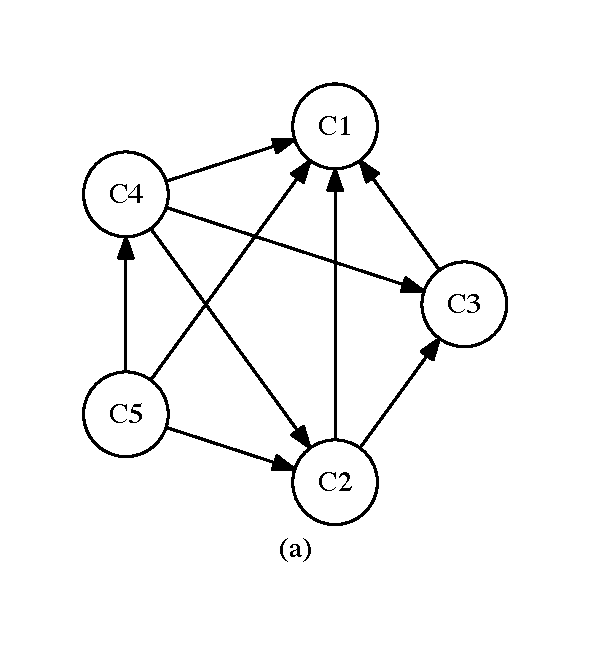
\includegraphics[width=0.42\columnwidth]{graphs/cart.pdf}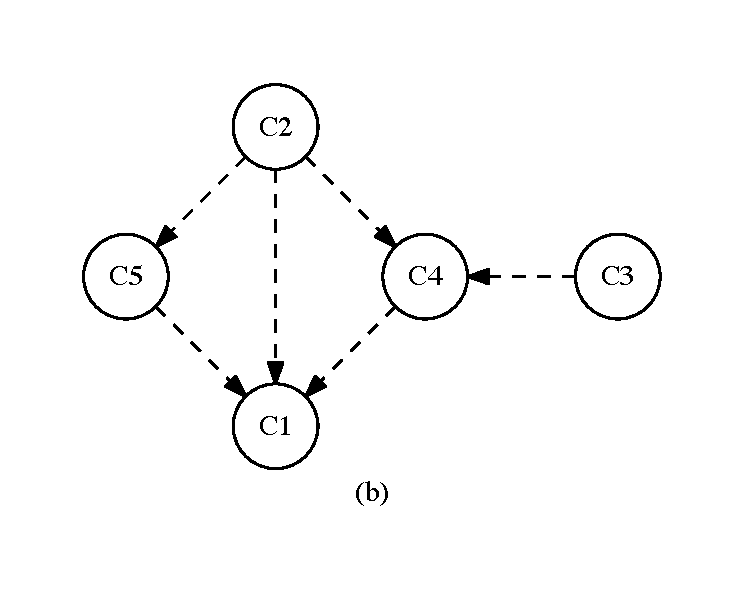
\includegraphics[width=0.57\columnwidth]{graphs/ccom.pdf}
\caption{Trend graphs for the CCC equivalence graph. Solid lines represent the artifact analysis. Dashed lines represent the understandability analysis.}
\label{fig:graphsforanalysis}
\end{figure}

\subsubsection{Building the Graphs}
In the community standards graph, we represent a directed edge from $C2 \rightarrow C1$ when  nPatterns(C1) $>$ nPatterns(C2) \emph{and}  nProjects(C1) $>$ nProjects(C2). When there is a conflict between nPatterns and nProjects, as is the case between L2 and L3 where L2 is found in more patterns and L3 is found in more projects, an undirected edge is used. In the end, we have a graph, like the left-most one in Figure~\ref{fig:graphsforanalysis}a, representing the frequency trends among the community artifacts. Note that with the CCC group, there is no edge between C3 and C5 because there is no straightforward refactoring between those representations, as discussed in Section~\ref{}. 

In the understandability graph, we represent a directed edge from $C2 \rightarrow C1$ when match(C1) $>$ match(C2) \emph{and} compose(C1) $>$ compose(C2). When there is a conflict between match and compose, as is the case with T1 and T3 where match(T1) is higher but compose(T3) is higher, an undirected edge is used. When one metric has a tie, as is the case with compose(C1) = compose(C5), we resort to the matching to provide the direction, in this case, C5 $\rightarrow$ C1. An example understandability graph is provided in Figure~\ref{fig:graphsforanalysis}b with the dashed arrows.\footnote{When there are confounded representations, as is the case with E8, E4, and E5 which all use tranformations from the CCC and the LIT equivalence classes, we omit those from the understandability graph. This makes sense since all use a transformation between T1 and T4 strongly favoring T1. }

\subsubsection{Topological Sorting}
Once the graphs are built for each equivalence class and each set of metrics, community standards and understandability, we apply a modified version of Kahn's topological sorting algorithm to obtain a total ordering on the nodes. 

\begin{algorithm}
  \caption{Modified Topological Sort}\label{topological}
  \begin{algorithmic}[1]
\State  $L \gets$ []
\State $S \gets$ []
\State Remove all undirected edges
\State Add all disconnected nodes to $L$ and remove from graph. If there are more than one, mark the tie. \label{markTie1}
\State Add all nodes with no incoming edges to $S$
\While {$S$ is non-empty}
	\State remove a node $n$ from $S$ \label{setn}
	\State add $n$ to $L$ 
	\For {node $m$ such that $e$ is an edge from $n \rightarrow m$}
		\State remove $e$
		\If{$m$ has no incoming edges}
			\State add $m$ to $S$ \label{addToS}
		\EndIf
	\EndFor
	\State If multiple nodes were added to $S$ in this iteration, mark those as a tie \label{markTie2}
\EndWhile
\State For all ties in $L$, use a tiebreaker. 
  \end{algorithmic}
\end{algorithm}

One downside to Kahn's algorithm is that the total ordering is not unique. Thus, we mark ties in order to identify when a tiebreaker is needed to enforce a total ordering on the nodes. For example, on the understandability graph in Figure~\ref{fig:graphsforanalysis}b, there is a tie between C3 and C2 since both have no incoming edges, so they are marked as a tie on Line~\ref{markTie1}. Further, when $n=C2$ on line~\ref{setn}, both C5 and C4 are added to $S$ on Line~\ref{addToS}, thus the tie between them is parked on line~\ref{markTie2}. In these cases, a tiebreaker is needed. 

Breaking ties on the community standards graph comes down to choosing the representation that appears in a larger number of projects, since it is more widespread across the community. Breaking ties in the understandability graph is trickier. Using Table~\ref{table:testedEdgesTable}, we compute the average matching score for all instances of each representation, and do the same for the composition score. For example, C4 appears in E6, E2 and E9 with an overall average matching score of 0.81 and composition score of 24.3. C5 appears in E3 and E7 (we omit E8 as C5 is confounded with T1) with an average matching of 0.87 and composition of 28.28. Thus, C5 is favored to C4 and appears higher in the sorting. 

After running the topological sort in Algorithm~\ref{topological}, we have a total ordering on nodes for each graph. After breaking ties as described, the topological sorts for all graphs are shown in Table~\ref{topologicalResults}. 

\begin{table*}
\centering
\caption{Topological Sorting, with the left-most position being highest \label{topologicalResults}}
\begin{tabular}{|| l || l || l || l || l || l ||}
				& CCC			& DBB 		& LBW & SNG & LIT \\ \hline
Community 		& C1 C3 C2 C4 C5 	& D2 D1 D3	&  L3 L2 L1 	& S2 S1 S3 	& T1 T3 T2 T4 \\  
Understandability 	& C1 C5 C4 C2 C3 	& D3 D1 D2 	& L3 L2		& S2 S1		& T1 T2 T4 T3 \\ 

\end{tabular}
\end{table*}

\subsubsection{Summary}
There is a clear winner in each equivalence class, with the exception of DBB. After rank 1 in the topological sort, it is not clear who the second place winner is in any of the classes. CCC and DBB are shuffled quite differently, and LBW and SNG don't have enough information from the understandability analysis since there is just one edge. DBB is an odd one as the orderings are completely reversed depending on the analysis. 

%\begin{figure}[tb]
%\centering
%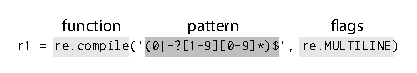
\includegraphics[width=\columnwidth]{illustrations/exampleUsage.eps}
%\vspace{-12pt}
%\caption{Example of one regex utilization}
%\vspace{-6pt}
%\label{fig:exampleUsage}
%\end{figure}








\paragraph{CCC Group}
This group is full of disagreement among the metrics. Five pairs were evaluated by all methods and only one pair, $C1 \Leftarrow C4$, has a somewhat clear winner with C1 (note that the matching metric is equivalent). All the others have disagreement between the community and understandability, or between the understandability metrics, matching and composition. 


\paragraph{DBB Group}
D2 has the most community support appearing in nearly 14\% of the patterns, yet the understandability metrics favor both D1 and D3 over D2. The results are consistent across the board that D3 is always favorable to D1. 

\paragraph{LWB Group}

\paragraph{LIT Group}

\paragraph{SNG Group}





%
%(for rough draft...)
%
%Looks like M6 and M8 are the best meta-refactorings according to ANOVA.
%If you peek at MTResults Processing.csv on google docs, M6 has the best refactoring...every OCTAL type should be converted to an OR or preferably a CCC.
%
%M8 has a weak P value, but still ok in one case (0.12) and consistently says that 'aa*' should be written as 'a+'.
%
%Looks like M0, M1, M2, M3 and M9 are very dependent on the regex chosen, so regex-specific refactorings like:
%0.1401 \verb!&d([aeiou][aeiou])z'    &d([aeiou]{2})z'!
%0.075   \verb![\t\r\f\n ]'    [\s]'!
%0.1024  \verb![a-f]([0-9]+)[a-f]' [a-f](\d+)[a-f]'!
%0.1271  \verb![\{][\$](\d+[.]\d)[}]'!
%\verb!\\\{\\\$(\d+\.\d)\}'!
%(from M0,M1,M2,M9 respectively)
%
%have okay P-values and may indicate regex-specific refactorings, but do not indicate an overall trend for that type of refactoring.
%Notice that M3 does not even have a strong p-value candidate, but this may be thrown off because of the very confusing regex chosen for CCC:
%0.78    0.79
%\verb!xyz[_\[\]`\^\\]'!    \verb!xyz[\x5b-\x5f]'!
%which has a lot of escape characters, so that the hex group was easier to understand than the CCC.
%
%
%
%Meanwhile M4,M5 and M7 have both ambiguous p-values and anova results.  But this is still a finding: that no refactoring is needed between things like:
%\verb!(q4fab|ab)'! (\verb!(q4f){0,1}ab)'!
%\verb!tri[abcdef]3'!   \verb!tri(a|b|c|d|e|f)3'!
%\verb!&(\w+);'!    \verb!&([A-Za-z0-9_]+);'!
%(from M4,M5,M7 respectively)
%
%Although one refactoring from M5 might be of slight interest:
%0.1196  FALSE   \verb!tri[a-f]3'!  \verb!tri(a|b|c|d|e|f)3'!

%\todoMid{more data from the composition problems}

\begin{table}\begin{small}\begin{center}\caption{some Group table caption}\label{table:groupANOVATable}\begin{tabular}
{lcc}
group & Pregex & Prefactoring \\
\toprule[0.16em]
CCC-LIT & 0.000000001 & 0.000030400\\
CCC & 0.000000000 & 0.427400000\\
DBB & 0.591100000 & 0.072200000\\
LIT & 0.000000000 & 0.000105000\\
LWB & 0.989700000 & 0.041200000\\
SNG & 0.000037600 & 0.958000000\\
\bottomrule[0.13em]\end{tabular}\end{center}\end{small}\end{table}

\section{Discussion}
\label{sec:discussion}
Based on our studies, we have identified preferred regex representations that may make regexes easier to understand than their smelly counterparts. Here, we summarize the results.

%We identify smells, not all refactorings are possible or advisable. See Equiv. class definitions for example limitations.

\subsection{Implications}
Our goal in this work was to identify code smells in regular expressions.
In an evaluation using humans where we measure comprehension of various regular expressions, we find that it is easier to understand regexes that do not use hex or octal characters,
that repetition operators, such as \verb!?! in D2 can decrease comprehension, and that using ranges is preferred to some character classes (e.g., \verb![A-Za-z0-9_! is often more understandable than \verb!\w!).

In general, the factors that explain differences in comprehension metrics are the DFA size and the representation, where DFA sizes range from two to eight and the representations are as defined in Section~\ref{fig:refactoringTree}.
The implications of these results are for refactoring tool designers and code maintainers. Opting to use the preferred regex representations, when possible, may increase the understandability of regexes in source code.
Since there are differences in regex comprehension based on how regexes are syntactically composed, it also has implications for refactoring tool designers to add refactoring for comprehension, which could enable developers to more easily compose regexes that are easier to understand.
%In the CCC equivalence class, C1 (e.g., \verb![0-9a]!) is more commonly found in the patterns and projects. C2 (e.g., \verb![0123456789a]!) and C3 (e.g., \verb![^\x00-/:-`b-\x7F]!) appear in similar percentages of patterns and projects but there is no significant difference in understandability considering two pairs of regexes tested.
%A small preference is shown for C1 over C2, indicating ranges in character classes enhance comprehension.
%% Regex length is probably important for understandability, though we did not test for this.
%
%% - the longest regex in the corpus is \todoNow{X} characters long...
%%Anyway C2 is common but less readable. C4 is somewhat less common to use default in CC - why? C5 is rare, but marginally more readable than C2. Not enough data or contrast to come to a conclusion about C3 - it is a catch-all?
%
%In DBB, D3 (e.g., \verb!pBs|pBBs|pBBBs!) merits further exploration because it is the most understandable but least common node in the group. This may be because explicitly listing the possibilities with an OR is easy to grasp, but if the number of items in the OR is too large, understandability may suffer. Further analysis is needed to determine the optimal thresholds for representing a regex as D3 compared to D1 (e.g., \verb!pB{1,3}s!) or D2 (e.g., \verb!pBB?B?s!).
%%Intuitively, it seems that D2 may be more common because 0,1 is just a more common use case than an arbitrary range like 4, 25.
%
%In the SNG group, S1 is compact (e.g., \verb!S{3}!), but S2 was preferred (e.g., \verb!SSS!). Similar to DBB, this may be due to the particular examples chosen in the analysis, as a large number of explicit repetitions may not be as preferred.
%
%In LWB, L2 (e.g., \verb!AAA*!) and L3 (e.g., \verb!AA+!) appear in similar numbers of patterns and projects, but comprehension favors L3.
%% , it's clear that this is a rare use case, and also that L3 is the most common use case. Patterns using star are secondary, helper patterns because they will trivially match anything, so they are less common. But anyway...
%
%
%% is nice, but
%%so probably better than S2. S2 is over-weighted because of double-characters in regular words like foot.
%In the LIT group, T1 (e.g., \verb!\a\$>!) is the typical way to list literals, but the reason to use hex (T2) or oct (T4) types is because some characters cannot be represented any other way, such as unprintable chars. One main result of our work is that T4 (e.g., \verb!\007\036\062!) is less understandable than T2 (e.g., \verb!\x07\x24\x3E!), so if unprintable chars are required, hex is more understandable.
%%Regarding T3 (e.g., \verb!\a[$]>!), initially we thought the square brackets would be more understandable than using an escape character, but we found the opposite.
%Also, given a choice between T1 and T3, the escape character was more understandable.

\subsection{Opportunities For Future Work}
\label{sec:futureequivclasses}
%There are several directions for future work related to regex study and refactoring.
%
\noindent \textbf{Equivalence Class Models:}
We looked at five types of equivalence classes, each with three to five representations.
Future work could consider models with more types of equivalence classes, such as:
%For example, we have looked at all ranges as equivalent, all defaults as equivalent, and relied on many such generalizations. However, the range \verb![a-f]! is likely to be more understandable for most people than a range like \verb![:-`]!.
%In addition to breaking our 5 groups into more specific nodes, future work could model refactorings outside of these groups.
%
%We have not determined a list of all possible refactoring groups given the functional variety and significant number of features to consider, but we are aware of a few additional equivalence classes outside of our 5 groups, such as:
%Additional equivalence groups to consider may include:
\begin{itemize}[leftmargin=8pt] %\itemsep -2pt
%\item Single line option \verb!'''(.|\n)+'''! $\equiv$ \verb!(?s)'''(.)+'''!
\item Multiline option: { \verb!(?m)G\n! $\equiv$ \verb!(?m)G$!}
\item Case insensitive: { \verb!(?i)[a-z]! $\equiv$ \verb![A-Za-z]!}
\item Backreference: { \verb!(X)q\1! $\equiv$ \verb!(?P<name>X)q\g<name>!}
%\item Backreference: \texttt{ (X)q\textbackslash{}1 $\equiv$ (?P<name>X)q\textbackslash{}g<name>}
%\item Word Boundaries \verb!\bZ! $\equiv$ \verb!((?<=\w)(?=\W)|(?<=\W)(?=\w))Z!
\end{itemize}

There also may exist critical comprehension differences within a representation. For example, between C1~(e.g.,~\verb![0-9a]!) and C4 (e.g., \verb![\da]!), it could be that \verb![0-9]! is preferred to \verb![\d]!, but \verb![A-Za-z0-9_]! is not be preferred to \verb![\w]!.
By creating a more granular model of equivalence classes and carefully evaluating alternative representations of the most frequently used specific patterns, additional useful smells could be identified.

\noindent \textbf{Automated Improvement:}
Currently the equivalence classes are identified manually. In future work, we will consider automatically generating the equivalence classes by building behavioral clusters and observing how regex representations differ within those clusters. % and make recommendations according to the representations in each equivalence class.

%We focused on refactorings within a group, treating groups as orthogonal to one another. It would be interesting to see if there is some cooperation between pairs of edges in separate groups by applying more than one type of refactoring at once.
\iffalse
\noindent \textbf{Community-specific Comprehension:}
A straightforward way to assess understandability is to directly ask software professionals which regexes they prefer and why.
In our evaluation, we did not focus on a specific community or a specific regex purpose (e.g., validating e-mail address, validating IP-address, parsing URLs).
% but at least one side of the refactoring was contrived and we did not focus on any specific community (the 1544 projects we obtained regexes from were randomly obtained).
 If an understandability study used regexes sampled from the codebase of a specific community (e.g., most frequently observed regexes, most buggy regexes, regexes on the hottest execution paths, etc.), and measured the understanding of programming professionals working in that community, then the measurements and the refactoring they imply would be more likely to have a direct impact.
 \fi
%
%In another study, we did a survey where software professionals indicated that understandability of regexes they find in source code is a major pain point. In this study, our participants indicated that they read about twice as many regexes as they compose. What is the impact on maintainers, developers and contributors to open-source projects of not being able to understand a regex that they find in the code they are working with? Presumably this is a frustrating experience - how much does a confusing regex slow down a software professional? What bugs or other negative factors can be attributed to or associated with regexes that are difficult to understand? How often does this happen and in what settings? Future work could tailor an in-depth exploration of the overall costs of confusing regexes and the potential benefits of refactoring or other treatments for confusing regexes.

%\vspace{-1pt}
%\paragraph{Regex Migration Libraries}
%We have identified opportunities
% to improve the understandability of regexes in existing code bases by looking for some of the less understandable regex representations, which can be thought of as antipatterns, and refactoring to the more common or understandable representations.
% Building migration libraries is a promising direction of future work to ease the manual burden of this process, similar in spirit to prior work on class library migration~\cite{Balaban:2005:RSC:1103845.1094832}.
%
%%\paragraph{Regex Refactoring Applications}
%%Maintainers of code that is intentionally obfuscated for security purposes may want to develop regexes that they understand and then automatically transform them into the least understandable regex possible.
%%
%%One fundamental concept that many users of regex struggle to learn is when to use regexes for simple parsing, and when to write a full-fledged parser (for example, when parsing HTML). Regexes that are trying to parse HTML, XML or similar languages could be refactored not into a better regex, but into some code with an equivalent intention that does parsing much better.
%
%%\vspace{-1pt}
%%\paragraph{Regex Programming Standards}
%%Many organizations enforce coding standards in their repositories to ease understandability.
%%Presently, we are not aware of coding standards for regular expressions, but this work suggests that enforcing standard representations for various regex constructs could ease comprehension.
%
%\vspace{-1pt}
%\paragraph{Regex Refactoring for Performance}
%The representation of regexes may have a strong impact on the runtime performance of a chosen regex engine. Prior work has sought to expedite the processing of regexes over large bodies of text~\cite{Baeza-Yates:1996:FTS:235809.235810}.
%Refactoring regexes for performance would complement those efforts.
%%Further study is needed to determine which representations are most efficient, leading to a whole new area of study on regex refactoring for performance, a topic already explored for
%%Depending on the efficiency of an organization's chosen regex engine, an organization may want to enforce standards for efficiency.
%%, or for compatibility with a regex analysis tool like Z3, HAMPI, BRICS or REX.

\subsection{Threats to Validity}

\noindent \textbf{Internal:}
We measure understandability using two metrics: matching and composition. These measures may not reflect the actual understanding of regex behavior. To mitigate, we used multiple metrics that require reading and writing regexes. %, but the threat remains.

We measure community support using two metrics: patterns and projects. These measures may not reflect the actual desire of the community to use the representations contained within. To mitigate, we use multiple metrics.

Participants evaluated regular expressions on MTurk, which may not be reflective enough of the context in which programmers would encounter regexes in practice. Further study is needed to determine the impact of the experimental context.

Some regex representations from the equivalence classes were not involved in the understandability analysis and that may have biased the results against those nodes.
More complete coverage of the edges in the equivalence classes is needed.

We treated unsure responses as omissions that did not count against the matching scores. Thus, if a participant answered two strings correctly and marked the other three strings as unsure, then this was 2/2 correct, not 2/5. This may have inflated the matching scores, however, less than 5\% of the matching scores were impacted by such responses.





%
%In our analyses, we measure understandability using matching and composition metrics.
%However, there may be other ways to approach regex understandability, such as deciding which regexes in a set are equivalent, finding the minimum modification to some text so that a given regex will match it.
%It may also be meaningful to provide some code that exists around a regex as context since that would better represent a scenario in which programmers would encounter regexes in practice.
%Further study is needed to determine if the chosen metrics and experimentation context have resulted in a reasonable measure of understandability.

\noindent \textbf{External:}
The regexes used in the evaluation were inspired by those found in Python code, which is just one language that has library support for regexes, and may not generalize to other languages. %Furthermore, the DFAs and regex string length are not the main consideration during MTurk study. The DFAs for the regexes ranged in size from two to eight, so the comprehension metrics may not generalize to larger regexes.
Furthermore, the DFAs for the regexes ranged in size from two to eight, so the comprehension metrics may not generalize to larger regexes.% Thus, we may have missed opportunities for other refactorings based on how programmers use regexes in other programming languages.

%While we identify code smells, not all code smells are removable through refactoring. For example, between T4 and T1, if the regex matches on non-printable characters, a transformation to T1 is not possible. Similarly, the regex \verb![2-9]! in C1 cannot transform to C4 since there does not exist a default character class with the same behavior (i.e., \verb![0-9]! $\equiv$ \verb![\d]!).

Our criteria for membership in a representation may overestimate the opportunities for refactoring to address the smells. For example, \verb![a-f]! in C1 cannot be refactored to C4 since there does not exist a default character class for that range of characters. The transformation between T4 and T1 may not be possible if the regex matches on non-printable characters, which require hex or octal representation. A finer-grained analysis is needed to identify actual refactoring opportunities from the smells.

Participants in our survey came from MTurk, which may not be representative of people who read and write regexes on a regular basis. However, all participants demonstrated knowledge of regexes through a qualification test. Our survey are done online without supervision and cheating could also be a factor impacting the results.


The results of the understandability analysis may be closely tied to the particular regexes chosen for the experiment. For many of the representations, we had several comparisons. Still, replication with more regex patterns is needed.% to validate our results.



%\todoMid{what about the threat of too few examples per node? Didn't cover every edge. Regex set is randomly collected online, not focused on any specific target audience.}

%Our community analysis only focuses on the Python language, but as the vast majority of regex features are shared across most general programming languages (e.g., Java, C, C\#, or Ruby), a Python {pattern} will (almost always) behave the same when used in other languages and our results are likely to generalize.
%, whereas a utilization is not universal in the same way (i.e., it may not compile in other languages, even with small modifications to function and flag names).
%As an example, the {\tt re.MULTILINE} flag, or similar, is present in Python, Java, and C\#, but the Python {\tt re.DOTALL} flag is not present in C\# though it has an equivalent flag in Java.


\section{Related Work}

\todoMid{We are building on the survey that indicates regexes are hard to read, and the apparent lack of any regex readability refactoring attempts.  Many papers have talked about refactoring, basically it is changing the form but not the behavior.}



\section{Conclusion}
\label{sec:conclusion}
In an effort to find smells that impact regex understandability, we created five types of equivalence class models and used these models to investigate the most common representations and most comprehensible representations per class. 
%We found the most common representations per class by both number of patterns and number of projects to be C1, T1 and S2. 
%We identified three strongly preferred transformations between representations (i.e., $\overrightarrow{T4 T1}$, $\overrightarrow{D2 D3}$, and $\overrightarrow{L2 L3}$). 
The high agreement between the community standards and understandability analyses suggests that one particular representation can be preferred over others in most cases. 
Based on these results, we recommend using hex to represent unprintable characters in regexes instead of octal and using escape special characters with slashes instead of wrapping them in brackets. Further research is needed into more granular models that treat common specific cases separately. %and that address the effect of length on understandability when transforming from one representation to another.








\balance

\section*{Acknowledgements}
This work is supported in part by  NSF SHF-EAGER-1446932.


\bibliographystyle{IEEEtran}
\bibliography{biblio,stolee}

\end{document}

